\chapter{变分视角：从 VAE 到 DDPM}\label{ch:variational}


本章中，我们从变分的视角来审视扩散模型。我们首先介绍变分自编码器（Variational Autoencoders，VAE），它用隐变量表示数据，并通过最大化对数似然的一个可处理的下界来进行训练。在这一设定下，学习到的编码器将观测映射到隐变量，学习到的解码器将隐变量映射回观测，从而闭合建模回路。

在这一模式的基础上，层次化变体（层次化 VAE，Hierarchical VAEs）堆叠多层隐变量以捕捉多尺度的结构。在这种设定下，去噪扩散概率模型（Denoising Diffusion Probabilistic Models，DDPM）遵循同样的模板：它不再联合训练编码器和解码器，而是将编码器固定为一个前向加噪过程，逐步将数据映射为噪声，训练则学习一个解码器，通过连续的去噪步骤反转这条路径。从这个角度看，VAE、层次化 VAE 和扩散模型都在优化一个由变分界定义的似然代理量，为这里介绍的方法提供了共同的基础。





\newpage
\section{变分自编码器}\label{sec:vae}
神经网络如何学会生成逼真的数据？
一个自然的出发点是\emph{自编码器}（autoencoder），它由两个网络组成：
一个确定性的\emph{编码器}，将输入压缩为低维隐编码；以及一个确定性的\emph{解码器}，从该编码重建输入。
训练过程最小化原始输入与其重建之间的重建误差。
虽然这种设定能够实现精确的重建，但隐空间是无结构的：随机采样隐编码通常会产生无意义的输出，从而限制了模型在生成任务中的用途。



% How can a neural network learn to generate realistic data? A natural starting point is the autoencoder, a framework \se{introduce networks (encoder, decoder) first, then discuss how they are trained} trained to reconstruct inputs through a low dimensional latent representation. A deterministic encoder compresses the input into a latent code, which a deterministic decoder then uses to reconstruct the original data. While this setup enables faithful reconstruction, it lacks a structured latent space. As a result, decoding randomly sampled latent codes typically yields meaningless outputs, making the model ineffective for generation.

\emph{变分自编码器（VAE）}\citep{kingma2013auto}  通过在隐空间上施加概率结构来解决这一问题。这将模型从一个简单的重建工具转变为一个真正的生成模型，能够产生新颖而逼真的数据。



\subsection{概率编码器与解码器}

\begin{figure}[tbh!]
\centering
\resizebox{0.85\linewidth}{!}{%
\begin{tikzpicture}[>=Latex, thick, font=\sffamily, node distance=0.8cm]

\tikzset{
  state/.style={
    rectangle, rounded corners=3pt,
    draw=black, fill=gray!10,
    minimum height=45pt, minimum width=25pt, align=center,
    % Add outer sep to ensure arrows connect cleanly to the rounded edges
    outer sep=0pt 
  },
  latent/.style={
    rectangle, rounded corners=3pt,
    draw=black, fill=gray!10,
    minimum height=28pt, minimum width=28pt, align=center,
    outer sep=0pt
  },
  encoderblock/.style={
    trapezium, trapezium stretches=true,
    % Adjust angles to create the frustum shape.
    % The 'top' and 'bottom' here refer to the sides that become the vertical parallels after rotation.
    trapezium left angle=80,  % Closer to 90 for less slope
    trapezium right angle=80, % Closer to 90 for less slope
    shape border rotate=270,   % Rotate 90 degrees clockwise for vertical parallels
    draw=black, fill=gray!20,
    minimum height=8pt, minimum width=15pt, inner sep=4pt, align=center
  },
  decoderblock/.style={
    trapezium, trapezium stretches=true,
    trapezium left angle=80,
    trapezium right angle=80,
    shape border rotate=90,  % Rotate 270 degrees clockwise (or -90)
    draw=black, fill=gray!20,
    minimum height=8pt, minimum width=15pt, inner sep=4pt, align=center
  }
}

% nodes
\node[state] (x) {$\mathbf{x}$};
\node[encoderblock, right=of x] (enc) {\footnotesize\textbf{编码器}\\[-2pt]
 \footnotesize $q_{\bm{\theta}}(\mathbf{z}|\mathbf{x})$}; % Using bm for bold math
\node[latent, right=of enc] (z) {$\mathbf{z}$};
\node[decoderblock, right=of z] (dec) {\footnotesize\textbf{解码器}\\[-2pt]
  \footnotesize$p_{\bm{\phi}}(\mathbf{x}|\mathbf{z})$}; % Using bm for bold math
\node[state, right=of dec] (xprime) {$\mathbf{x}'$};

% short arrows (edge-to-edge)
\draw[->] (x) -- (enc); % Changed to direct node-to-node, TikZ usually finds the nearest edge
\draw[->] (enc) -- (z);
\draw[->] (z) -- (dec);
\draw[->] (dec) -- (xprime);

\end{tikzpicture}}
\caption{\textbfs{VAE 示意图。}它由一个随机编码器 $q_{\bm{\theta}}(\rvz|\rvx)$（将数据 $\rvx$ 映射到隐变量 $\rvz$）和一个解码器 $p_{\bm{\phi}}(\rvx|\rvz)$（从隐变量重建数据）组成。\figcredit{由作者绘制。}}
\label{fig:vae-graph}
\end{figure}

\paragraph{解码器（生成器）的构造。}

% Our objective is to model the data generation process. VAE assumes that each observation $\mathbf{x}$ is generated from a latent variable $\mathbf{z}$ drawn from a simple \emph{prior distribution}, typically standard Gaussian: $\mathbf{z} \sim p_{\text{prior}} := \mathcal{N}(\mathbf{0}, \mathbf{I})$. More precisely, we define a \emph{decoder (generator)} network $p_{\bm{\phi}}(\mathbf{x}|\mathbf{z})$, which learns to generate data from latent inputs $\rvz$. New samples are generated by first sampling $\mathbf{z} \sim p_{\text{prior}}$ and then decoding via $\mathbf{x} \sim p_{\bm{\phi}}(\mathbf{x}|\mathbf{z})$.

% \se{need to say the decoder is simple, like a gaussian or fully factor. also probably give some intuition? maybe something along the lines that generating pixels is hard, but it becomes easier if we have a bunch of features (latent vars) that describe content, colors, etc}

% The VAE defines a latent-variable generative model via the marginal likelihood:
% \[
% p_{\bm{\phi}}(\mathbf{x}) = \int p_{\bm{\phi}}(\mathbf{x}|\mathbf{z}) p(\mathbf{z}) \mathrm{d}\mathbf{z}.
% \]
% Ideally, the decoder parameters $\bm{\phi}$ would be learned by maximizing the marginal likelihood of the observed data, as in maximum likelihood training (see \Cref{eq:MLE}). However, this objective is generally intractable for expressive, non-linear decoders, since the marginalization over latent variables $\mathbf{z}$ lacks a closed-form solution. As a result, direct MLE becomes computationally infeasible.
在 VAE 中，我们区分两类变量：
\emph{观测变量} $\rvx$，对应我们看到的数据（例如一张图像），
以及\emph{隐变量} $\rvz$，它捕捉隐藏的变化因素
（例如物体的形状、颜色或风格）。
该模型假设每个观测 $\rvx$ 都由一个从简单的\emph{先验分布}（通常是标准高斯分布）中采样得到的隐变量生成，
即 $\rvz \sim p_{\text{prior}} := \mathcal{N}(\mathbf{0}, \mathbf{I})$。

为了将 $\rvz$ 映射回数据空间，我们定义一个\emph{解码器（生成器）}分布
$p_{\bm{\phi}}(\rvx|\rvz)$。在实践中，这个解码器保持简单，通常是因式分解的高斯分布
（见 \Cref{subsec:optimization-vae}）或类似分布，以便学习专注于提取
有用的隐特征，而非记住数据。
直观地说，逐像素地直接生成像素极其困难；相反，
隐变量提供了一种紧凑的表示，
从它出发解码出精确的像素排列要容易得多。
新样本的生成方式是：先采样 $\rvz \sim p_{\text{prior}}$，
然后通过 $\rvx \sim p_{\bm{\phi}}(\rvx|\rvz)$ 解码。

因此，VAE 通过边际似然定义了一个隐变量生成模型：
\[
p_{\bm{\phi}}(\rvx) = \int p_{\bm{\phi}}(\rvx|\rvz) p(\rvz) \diff \rvz.
\]
理想情况下，解码器参数 $\bm{\phi}$ 通过最大化这一边际似然来学习，
如同极大似然估计那样（见 \Cref{eq:MLE}）。
然而，由于对 $\rvz$ 的积分对于表达能力强的非线性解码器是不可处理的，
直接的 MLE 在计算上不可行，这促使了 VAE 中所使用的变分方法。

% \se{i think you need to use some text to clearly explain the difference between observed and latent vars at the beginning}



\paragraph{编码器（推断网络）的构造。}
% To get a handle on our intractable generator, we might try to reverse the process: given a real data point $\mathbf{x}$, what distribution of latent codes $\mathbf{z}$ could have been its origin? The formal answer is given by Bayes' rule:
% \[
% p_{\bm{\phi}}(\mathbf{z}|\mathbf{x}) = \frac{p_{\bm{\phi}}(\mathbf{x}|\mathbf{z})p(\mathbf{z})}{p_{\bm{\phi}}(\mathbf{x})}.
% \]
% But this brings us to a second, related impasse. The denominator is $p_{\bm{\phi}}(\mathbf{x})$, the very intractable likelihood that halted our progress in the first place. We are in a computational catch: to train our generator, we need to solve an inference problem that itself requires a trained generator. \se{this is confusing. the generator doesn't have to be trained.}

% This is where the ``variational'' in VAE makes its brilliant entrance. \se{brilliant is inappropriate. keep scientific language as dry/objective as possible}
% Instead of calculating this ideal mapping exactly, we learn to \emph{approximate} it. We introduce a second neural network, the \emph{encoder} $q_{\bm{\theta}}(\mathbf{z}|\mathbf{x})$, and give it a crucial job: act as a tractable and learnable proxy for the intractable true mapping.
% \[
% q_{\bm{\theta}}(\mathbf{z}|\mathbf{x}) \approx p_{\bm{\phi}}(\mathbf{z}|\mathbf{x}).
% \]
% This encoder  takes in real data and outputs a distribution over the latent space, providing the essential, workable link from $\mathbf{x}$ back to $\mathbf{z}$ that we need to build our objective. \se{wording is a bit odd}


为了将我们不可处理的生成器与真实数据联系起来，考虑反向问题：
给定一个观测 $\rvx$，什么样的隐编码 $\rvz$ 可能产生了它？
由贝叶斯法则，后验分布为
\[
p_{\bm{\phi}}(\rvz|\rvx) \;=\; \frac{p_{\bm{\phi}}(\rvx|\rvz) p(\rvz)}{p_{\bm{\phi}}(\rvx)}.
\]
困难在于分母涉及边际似然 $p_{\bm{\phi}}(\rvx)$，
它需要对所有隐变量积分，对于非线性解码器是不可处理的。
因此，从 $\rvx$ 精确推断 $\rvz$ 在计算上是不可行的。

VAE 中的“变分”步骤通过用一个可处理的近似来代替不可处理的后验来解决这一问题。
我们引入一个\emph{编码器}（或推断网络）$q_{\bm{\theta}}(\rvz|\rvx)$，由神经网络参数化，
其作用是充当一个可学习的代理：
\[
q_{\bm{\theta}}(\rvz|\rvx) \;\approx\; p_{\bm{\phi}}(\rvz|\rvx).
\]
在实践中，编码器将每个观测数据点 $\rvx$ 映射到隐编码上的一个分布，
提供了一条从 $\rvx$ 回到 $\rvz$ 的可行且可训练的路径，从而支持学习。




\subsection{通过证据下界（ELBO）进行训练}

现在我们定义一个可计算的训练目标。虽然我们无法直接优化 $\log p_{\bm{\phi}}(\mathbf{x})$，但我们可以最大化它的一个下界——即\emph{证据下界（Evidence Lower Bound，ELBO）}：

\thmp{证据下界（ELBO）}{elbo}{
对于任意数据点 $\mathbf{x}$，对数似然满足：
\[
\log p_{\bm{\phi}}(\mathbf{x}) \geq \mathcal{L}_{\text{ELBO}}(\bm{\theta}, \bm{\phi}; \mathbf{x}),
\]
其中 ELBO 由下式给出： 
\begin{align}\label{eq:vae-elbo}
    \mathcal{L}_{\text{ELBO}} = \underbrace{\mathbb{E}_{\mathbf{z} \sim q_{\bm{\theta}}(\mathbf{z}|\mathbf{x})} \left[ \log p_{\bm{\phi}}(\mathbf{x}|\mathbf{z}) \right]}_{\text{Reconstruction Term}} - \underbrace{\mathcal{D}_{\mathrm{KL}}\left( q_{\bm{\theta}}(\mathbf{z}|\mathbf{x}) \| p(\mathbf{z}) \right)}_{\text{Latent Regularization}}.
\end{align}
}{
ELBO 来源于 Jensen 不等式：
\begin{align*}
\log p_{\bm{\phi}}(\mathbf{x}) &= \log \int p_{\bm{\phi}}(\mathbf{x}, \mathbf{z})   \mathrm{d}\mathbf{z} = \log \int q_{\bm{\theta}}(\mathbf{z}|\mathbf{x}) \frac{p_{\bm{\phi}}(\mathbf{x}, \mathbf{z})}{q_{\bm{\theta}}(\mathbf{z}|\mathbf{x})}   \mathrm{d}\mathbf{z} \\
&= \log \mathbb{E}_{\mathbf{z} \sim q_{\bm{\theta}}(\mathbf{z}|\mathbf{x})} \left[ \frac{p_{\bm{\phi}}(\mathbf{x}, \mathbf{z})}{q_{\bm{\theta}}(\mathbf{z}|\mathbf{x})} \right] \geq \mathbb{E}_{\mathbf{z} \sim q_{\bm{\theta}}(\mathbf{z}|\mathbf{x})} \left[ \log \frac{p_{\bm{\phi}}(\mathbf{x}, \mathbf{z})}{q_{\bm{\theta}}(\mathbf{z}|\mathbf{x})} \right].
\end{align*}
}
ELBO 目标自然地分解为两部分：
\begin{itemize}
    % \item \textbfs{Reconstruction:} Encourages accurate reconstruction of $\mathbf{x}$ from $\mathbf{z}$. This objective arises naturally from a KL-based variational inequality. However, on its own, it merely memorizes the training data, motivating a second KL term to regularize the latent space for generative modeling.
    % \se{refer back to the  earlier autoencoder discussion}
    \item \textbfs{重建项：} 鼓励从隐编码 $\mathbf{z}$ 准确恢复 $\mathbf{x}$。在高斯编码器和解码器假设下，这一项恰好退化为自编码器所熟悉的重建损失（参见 \Cref{subsec:optimization-vae}）。然而，正如自编码器那样，仅优化这一项会有记住训练数据的风险，因此需要额外的正则化。
    \item \textbfs{隐变量 KL 项：} 鼓励编码器分布 $q_{\bm{\theta}}(\mathbf{z}|\mathbf{x})$ 保持接近一个简单的高斯先验 $p_{\mathrm{prior}}(\mathbf{z})$。这种正则化将隐空间塑造为光滑且连续的结构，确保从先验中采样的样本能够被可靠地解码，从而实现有意义的生成。
\end{itemize}
这种权衡既保证了忠实的重建，又保证了连贯的采样。

\paragraph{信息论视角：作为散度界的 ELBO。}
% The ELBO objective enjoys a deep connection to information theory. To understand this, we recall that MLE training is equivalent to minimizing the KL divergence
% \[
% \mathcal{D}_{\mathrm{KL}}(p_{\text{data}}(\rvx) \| p_{\bm{\phi}}(\rvx)),
% \]
% which measures how well the generative model approximates the true data distribution. However, this quantity is generally intractable. The variational framework offers a powerful workaround by introducing a joint comparison.

% Let us consider the two joint distributions induced by the decoder and the encoder:
% \begin{itemize}
%     \item The \textbfs{generative joint}, $p_{\bm{\phi}}(\mathbf{x}, \mathbf{z}) = p(\mathbf{z}) p_{\bm{\phi}}(\mathbf{x}|\mathbf{z})$, which represents the model’s generative process.
%     \item The \textbfs{inference joint}, $q_{\bm{\theta}}(\mathbf{x}, \mathbf{z}) = p_{\text{data}}(\mathbf{x}) q_{\bm{\theta}}(\mathbf{z}|\mathbf{x})$, which couples real data with its encoded latent.
% \end{itemize}
% Comparing these joints gives rise to the inequality
% \begin{align}\label{eq:joint-bound}
%     \mathcal{D}_{\mathrm{KL}}(p_{\text{data}}(\rvx) \| p_{\bm{\phi}}(\rvx)) \leq \mathcal{D}_{\mathrm{KL}}(q_{\bm{\theta}}(\mathbf{x}, \mathbf{z}) \| p_{\bm{\phi}}(\mathbf{x}, \mathbf{z})),
% \end{align}
% % \se{notations are a bit inconsistent (sometimes with arguments, sometimes not)}
% which follows from the \emph{Data Processing Inequality (DPI)} and is also known as the ``chain rule for KL divergence''. The intuition is that marginalizing the latent cause $\mathbf{z}$ to observe only the outcome $\mathbf{x}$ can obscure modeling discrepancies that are only revealed when comparing the full joint processes.
% \se{the DPI story doesn't seem fitting to me, it's usually in terms of mutual information}

% To make this precise, observe the decomposition:
% \begin{align*}
%     &\underbrace{\mathcal{D}_{\mathrm{KL}}(q_{\bm{\theta}}(\mathbf{x}, \mathbf{z}) \| p_{\bm{\phi}}(\mathbf{x}, \mathbf{z}))}_{\text{Total Error Bound}} 
%     \\=& \mathbb{E}_{q_{\bm{\theta}}(\mathbf{x}, \mathbf{z})} \left[ \log \frac{p_{\text{data}}(\mathbf{x}) q_{\bm{\theta}}(\mathbf{z}|\mathbf{x})}{p_{\bm{\phi}}(\mathbf{x}) p_{\bm{\phi}}(\mathbf{z}|\mathbf{x})} \right] \\=&\mathbb{E}_{p_{\text{data}}(\mathbf{x})} \left[ \log \frac{p_{\text{data}}(\mathbf{x})}{p_{\bm{\phi}}(\mathbf{x})} + \mathcal{D}_{\mathrm{KL}}\left( q_{\bm{\theta}}(\mathbf{z}|\mathbf{x}) \| p_{\bm{\phi}}(\mathbf{z}|\mathbf{x}) \right) \right] \\
%     \\=&  \underbrace{\mathcal{D}_{\mathrm{KL}}(p_{\text{data}} \| p_{\bm{\phi}})}_{\text{True Modeling Error}} + \underbrace{\mathbb{E}_{p_{\text{data}}(\mathbf{x})} \big[ \mathcal{D}_{\mathrm{KL}}( q_{\bm{\theta}}(\mathbf{z}|\mathbf{x}) \| p_{\bm{\phi}}(\mathbf{z}|\mathbf{x}) ) \big]}_{\text{Inference Error}}.
% \end{align*}
% This identity yields a valuable interpretation: the joint KL divergence decomposes into the marginal KL of interest and the expected discrepancy between the approximate and true posteriors. The latter is always non-negative, confirming the DPI.

% Moreover, observe that
% \[
% \log p_{\bm{\phi}}(\mathbf{x}) - \mathcal{L}_{\text{ELBO}}(\bm{\theta}, \bm{\phi}; \mathbf{x}) = \mathcal{D}_{\mathrm{KL}}\left( q_{\bm{\theta}}(\mathbf{z}|\mathbf{x}) \| p_{\bm{\phi}}(\mathbf{z}|\mathbf{x}) \right),
% \]
% so the ``inference error'' term corresponds precisely to the gap between the true log-likelihood and the ELBO. Therefore, when we train a VAE by maximizing the ELBO, we are explicitly minimizing the inference error. This shows that our practical training algorithm is directly optimizing a meaningful component of the overall information-theoretic bound on how well our model captures the true data distribution.



% \se{you could consider adding a mixture of gaussians (discrete latent) as an example too to build intuition for the mixture effect}



ELBO 目标有一个自然的信息论解释。
回想一下，极大似然训练等价于最小化 KL 散度
\[
\mathcal{D}_{\mathrm{KL}}(p_{\text{data}}(\rvx) \| p_{\bm{\phi}}(\rvx)),
\]
它衡量模型分布对数据分布的近似程度。
由于这一项一般是不可处理的，变分框架引入了一个联合比较。

具体而言，考虑两个联合分布：
\begin{itemize}
    \item \textbfs{生成联合分布}，$p_{\bm{\phi}}(\rvx, \rvz) = p(\rvz) p_{\bm{\phi}}(\rvx|\rvz)$，描述模型如何生成数据；
    \item \textbfs{推断联合分布}，$q_{\bm{\theta}}(\rvx, \rvz) = p_{\text{data}}(\rvx) q_{\bm{\theta}}(\rvz|\rvx)$，将真实数据与其推断出的隐变量耦合在一起。
\end{itemize}
比较这些分布得到不等式
\begin{align}\label{eq:joint-bound}
    \mathcal{D}_{\mathrm{KL}}(p_{\text{data}}(\rvx) \| p_{\bm{\phi}}(\rvx)) 
    \leq \mathcal{D}_{\mathrm{KL}}(q_{\bm{\theta}}(\rvx,\rvz) \| p_{\bm{\phi}}(\rvx,\rvz)),
\end{align}
有时被称为 KL 散度的链式法则。
直观地说，仅比较边际分布（$\rvx$）可能掩盖一些差异，
而这些差异只有在考虑完整的隐变量—数据联合分布时才会显现。

形式上，可以将联合 KL 展开为
\begin{align*}
    &\underbrace{\mathcal{D}_{\mathrm{KL}}(q_{\bm{\theta}}(\mathbf{x}, \mathbf{z}) \| p_{\bm{\phi}}(\mathbf{x}, \mathbf{z}))}_{\text{Total Error Bound}} 
    \\=& \mathbb{E}_{q_{\bm{\theta}}(\mathbf{x}, \mathbf{z})} \left[ \log \frac{p_{\text{data}}(\mathbf{x}) q_{\bm{\theta}}(\mathbf{z}|\mathbf{x})}{p_{\bm{\phi}}(\mathbf{x}) p_{\bm{\phi}}(\mathbf{z}|\mathbf{x})} \right] \\=&\mathbb{E}_{p_{\text{data}}(\mathbf{x})} \left[ \log \frac{p_{\text{data}}(\mathbf{x})}{p_{\bm{\phi}}(\mathbf{x})} + \mathcal{D}_{\mathrm{KL}}\left( q_{\bm{\theta}}(\mathbf{z}|\mathbf{x}) \| p_{\bm{\phi}}(\mathbf{z}|\mathbf{x}) \right) \right] \\
    \\=&  \underbrace{\mathcal{D}_{\mathrm{KL}}(p_{\text{data}} \| p_{\bm{\phi}})}_{\text{True Modeling Error}} + \underbrace{\mathbb{E}_{p_{\text{data}}(\mathbf{x})} \big[ \mathcal{D}_{\mathrm{KL}}( q_{\bm{\theta}}(\mathbf{z}|\mathbf{x}) \| p_{\bm{\phi}}(\mathbf{z}|\mathbf{x}) ) \big]}_{\text{Inference Error}},
\end{align*}
其中第一项是真实的建模误差，第二项是推断误差，即近似后验与真实后验之间的差距。后者始终非负，这解释了 \Cref{eq:joint-bound}。

最后，注意
\[
\log p_{\bm{\phi}}(\rvx) - \mathcal{L}_{\text{ELBO}}(\bm{\theta},\bm{\phi};\rvx) 
= \mathcal{D}_{\mathrm{KL}} \left(q_{\bm{\theta}}(\rvz|\rvx)\|p_{\bm{\phi}}(\rvz|\rvx)\right).
\]
因此推断误差恰好是对数似然与 ELBO 之间的差距。
最大化 ELBO 因此对应于直接减小推断误差，确保训练最小化整个界中有意义的一部分。



% \se{you could consider adding a mixture of gaussians (discrete latent) as an example too to build intuition for the mixture effect}



% \begin{figure}
%     \begin{center}
% \scalebox{0.8}{
% \begin{tikzpicture}[node distance=3cm and 4cm, auto, >=Stealth]

% % Nodes
% \node[draw, rounded corners, minimum height=1.3cm, minimum width=4cm] (minKL) 
%     {$\displaystyle \min_{\bm{\phi}} \mathcal{D}(p_{\text{data}} \| p_{\bm{\phi}}) $};
% \node[draw, rounded corners, minimum height=1.3cm, minimum width=5cm, right=of minKL] (maxLogLik) 
%     {$\displaystyle \max_{\bm{\phi}} \mathbb{E}_{p_{\text{data}}}[\log p_{\bm{\phi}}]$};

% \node[draw, rounded corners, minimum height=1.3cm, minimum width=4cm, below=2.5cm of minKL] (minJointKL)
%     {$\displaystyle \min_{\bm{\phi},\bm{\theta}} \mathcal{D}\big(q_{\bm{\theta}}(\rvx,\rvz) \| p_{\bm{\phi}}(\rvx,\rvz)\big)$};
% \node[draw, rounded corners, minimum height=1.3cm, minimum width=4cm, right=of minJointKL] (maxELBO) 
%     {$\displaystyle \max_{\bm{\phi},\bm{\theta}} \mathbb{E}_{p_{\text{data}}} \big[ \mathcal{L}_{\mathrm{ELBO}}(\theta,\phi; \rvx) \big]$};

% % Arrows and labels
% \draw[<->, thick] (minKL) -- (maxLogLik) node[midway, above]{ \Cref{eq:MLE}};
% \draw[<->, thick] (minJointKL) -- (maxELBO) node[midway, above]{ \Cref{eq:joint-elbo}};

% % Vertical connectors
% \draw[thick] ($(minKL.south) + (0,0)$) -- ($(minJointKL.north) + (0,0)$);
% \draw[thick] ($(maxLogLik.south) + (0,0)$) -- ($(maxELBO.north) + (0,0)$);

% % Vertical labels
% \node at ($(minKL)!0.5!(minJointKL)$) [left=0.3cm] {\parbox{2cm}{\centering Theorem 2.1.1 \\ \rotatebox{270}{\Large$\leq$}}};
% \node at ($(maxLogLik)!0.5!(maxELBO)$) [right=0.3cm] {\parbox{2cm}{\centering Theorem 2.1.2 \\ \rotatebox{270}{\Large$\leq$}}};

% \end{tikzpicture}
% }
% \end{center}
%     \caption{Relations between marginal KL minimization and likelihood maximization (top) and their tractable upper-bound joint latent-variable counterparts with ELBO (bottom).
% }
% \label{fig:elbo-joint}
% \end{figure}


\subsection{高斯 VAE}\label{subsec:optimization-vae}
VAE 的一种标准表述对编码器和解码器都采用高斯分布。
\paragraph{编码器部分。}
编码器 $ q_{\bm{\theta}}(\mathbf{z} | \mathbf{x}) $ 通常建模为如下的高斯分布：
\[
q_{\bm{\theta}}(\mathbf{z} | \mathbf{x}) := \mathcal{N}\left(\mathbf{z}; \bm{\mu}_{\bm{\theta}}(\mathbf{x}), \operatorname{diag}(\bm{\sigma}_{\bm{\theta}}^2(\mathbf{x}))\right),
\]
其中 $\bm{\mu}_{\bm{\theta}} : \mathbb{R}^D \to \mathbb{R}^d$ 和 $\bm{\sigma}_{\bm{\theta}} : \mathbb{R}^D \to \mathbb{R}_+^d$ 是编码器网络的确定性输出。
\paragraph{解码器部分。} 解码器通常建模为具有固定方差的高斯分布：
\[
p_{\bm{\phi}}(\mathbf{x}|\mathbf{z}) := \mathcal{N}\bigl(\mathbf{x}; \bm{\mu}_{\bm{\phi}}(\mathbf{z}), \sigma^2 \rmI\bigr),
\]
其中 $\bm{\mu}_{\bm{\phi}} : \mathbb{R}^d \to \mathbb{R}^D$ 是一个神经网络，$\sigma > 0$ 是控制方差的小常数。
 
在这一假设下，ELBO 中的重建项简化为
\[
\mathbb{E}_{q_{\bm{\theta}}(\mathbf{z} | \mathbf{x})} \left[\log p_{\bm{\phi}}(\mathbf{x} | \mathbf{z})\right]
= - \frac{1}{2\sigma^2} \mathbb{E}_{q_{\bm{\theta}}(\mathbf{z} | \mathbf{x})} \left[\|\mathbf{x} - \bm{\mu}_{\bm{\phi}}(\mathbf{z})\|^2\right] + C,
\]
其中 $C$ 是与 $\bm{\theta}$ 和 $\bm{\phi}$ 无关的常数。于是 ELBO 目标退化为：
\[
\min_{\bm{\theta}, \bm{\phi}}  \mathbb{E}_{q_{\bm{\theta}}(\mathbf{z} | \mathbf{x})} \left[ \frac{1}{2\sigma^2} \|\mathbf{x} - \bm{\mu}_{\bm{\phi}}(\mathbf{z})\|^2 \right]
+ \mathcal{D}_{\mathrm{KL}}\big(q_{\bm{\theta}}(\mathbf{z} | \mathbf{x}) \| p_{\mathrm{prior}}(\mathbf{z})\big),
\]
其中由于高斯假设，KL 项具有闭式解。因此训练 VAE 退化为最小化一个正则化的重建损失。

\subsection{标准 VAE 的缺陷}\label{sec:drawback_standard_VAE}
尽管 VAE 框架在理论上很有吸引力，但它有一个关键缺陷：它经常产生模糊的输出。

\paragraph{VAE 中模糊的生成结果。}
为了理解这一现象，考虑一个固定的高斯编码器 $ q_{\text{enc}}(\mathbf{z}|\mathbf{x}) $，以及形如
\[
p_{\text{dec}}(\mathbf{x}|\mathbf{z}) = \mathcal{N}(\mathbf{x}; \bm{\mu}(\rvz), \sigma^2 \rmI),
\]
其中 $ \bm{\mu}(\rvz) $ 表示解码器网络。对于任意编码器，优化 ELBO 退化为（至多差一个加性常数）最小化期望重建误差：
\[
\argmin_{\bm{\mu}} \mathbb{E}_{p_{\text{data}}(\mathbf{x})q_{\text{enc}}(\mathbf{z}|\mathbf{x})} \left[ \| \mathbf{x} - \bm{\mu}(\rvz) \|^2 \right].
\]
这是关于 $ \bm{\mu}(\rvz) $ 的一个标准最小二乘问题，其解由条件均值以闭式给出：
\[
\bm{\mu}^*(\mathbf{z}) = \mathbb{E}_{q_{\text{enc}}(\mathbf{x}|\mathbf{z})}[\mathbf{x}],
\]
其中 $ q_{\text{enc}}(\mathbf{x}|\mathbf{z}) $ 是编码器诱导的、给定隐变量时输入上的后验，由贝叶斯法则定义：
\[
q_{\text{enc}}(\mathbf{x}|\mathbf{z})
=
\frac{q_{\text{enc}}(\mathbf{z}|\mathbf{x})\, p_{\text{data}}(\mathbf{x})}{q_{\text{enc}}(\mathbf{z})},
\qquad
q_{\text{enc}}(\mathbf{z})
:=
\int q_{\text{enc}}(\mathbf{z}|\mathbf{x})\, p_{\text{data}}(\mathbf{x})\, \diff \mathbf{x}.
\]

最优生成器通过贝叶斯法则的一个等价形式为：
\[
\bm{\mu}^*(\mathbf{z})
=
\frac{\mathbb{E}_{p_{\text{data}}(\mathbf{x})}\!\left[q_{\text{enc}}(\mathbf{z}|\mathbf{x}) \cdot \mathbf{x}\right]}
{q_{\text{enc}}(\mathbf{z})}
=
\frac{\mathbb{E}_{p_{\text{data}}(\mathbf{x})}\!\left[q_{\text{enc}}(\mathbf{z}|\mathbf{x}) \cdot \mathbf{x}\right]}
{\mathbb{E}_{p_{\text{data}}(\mathbf{x})}\!\left[q_{\text{enc}}(\mathbf{z}|\mathbf{x})\right]}.
\]
现在假设两个不同的输入 $ \mathbf{x} \neq \mathbf{x}' $ 被映射到隐空间中重叠的区域，即 $ q_{\text{enc}}(\cdot|\mathbf{x}) $ 和 $ q_{\text{enc}}(\cdot|\mathbf{x}') $ 的支撑集相交。那么 $\bm{\mu}^*(\mathbf{z})$ 会对多个可能不相关的输入求平均，从而导致模糊、不独特的输出。这种对相互冲突模式的平均效应是 VAE 生成样本具有特征性模糊的一个根本原因。




\newpage
\subsection{（选读）从标准 VAE 到层次化 VAE}
为了对复杂数据建模，层次化变分自编码器（Hierarchical Variational Autoencoders，HVAE）
\citep{vahdat2020nvae} 通过引入隐变量的层次结构来增强 VAE。这种深层的、分层的结构使模型能够在多个抽象层次上捕捉数据特征，显著提升了表达能力，并映射了真实世界数据的组合性本质。
\vspace{0.3cm}
\begin{figure}[tbh!]
    \centering
\begin{tikzpicture}[
    ->, % Sets default arrow type
    >=Stealth, % Sets default arrowhead style
    node_dist/.style={right=1.7cm of #1}, % Style for node distance
    font=\small,
    thick
  ]

  % Define a style for the circular nodes
  \tikzset{state/.style={
      rectangle,
      rounded corners=3pt,
      draw=black,
      fill=gray!10,
      minimum height=35pt,
      minimum width=25pt
    }
  }

  % Place the nodes
  \node[state] (x) {$\rvx$};
  \node[state] (z1) [node_dist=x] {$\rvz_1$};
  \node[state] (z2) [node_dist=z1] {$\rvz_2$};
  \node (dots) [right=0.7cm of z2] {$\boldsymbol{\cdots}$};
  \node[state] (zT) [node_dist=dots] {$\rvz_L$};

  % Draw the arrows (edges) with labels
  
  % Inference path (top, q, forward) - Shifted up
  \path ([yshift=4.5pt]x.east)  edge node[above] {$q_{\bm{\theta}}(\rvz_1|\rvx)$} ([yshift=4.5pt]z1.west);
  \path ([yshift=4.5pt]z1.east) edge node[above] {$q_{\bm{\theta}}(\rvz_2|\rvz_1)$} ([yshift=4.5pt]z2.west);
  \path ([yshift=4.5pt]z2.east) edge ([yshift=4.5pt]dots.west);
  % --- CHANGED: Added pos=0.4 to shift label left ---
  \path ([yshift=4.5pt]dots.east) edge node[above, pos=0.4] {$q_{\bm{\theta}}(\rvz_L|\rvz_{L-1})$} ([yshift=4.5pt]zT.west);
  
  % Generative path (bottom, p, backward) - Shifted down
  \path ([yshift=-4.5pt]z1.west) edge node[below] {$p_{\bm{\phi}}(\rvx|\rvz_1)$} ([yshift=-4.5pt]x.east);
  \path ([yshift=-4.5pt]z2.west) edge node[below] {$p_{\bm{\phi}}(\rvz_1|\rvz_2)$} ([yshift=-4.5pt]z1.east);
  \path ([yshift=-4.5pt]dots.west) edge ([yshift=-4.5pt]z2.east);
  % --- CHANGED: Added pos=0.6 to shift label left ---
  \path ([yshift=-4.5pt]zT.west) edge node[below, pos=0.6] {$p_{\bm{\phi}}(\rvz_{L-1}|\rvz_L)$} ([yshift=-4.5pt]dots.east);

\end{tikzpicture}

    \caption{\textbfs{HVAE 的计算图。}它具有层次化结构，在多个隐层上堆叠了可训练的编码器和解码器。\figcredit{由作者绘制。}
}
    \label{fig:hvae-graph}
\end{figure}


\paragraph{HVAE 的建模。}
与使用单一隐编码 $\mathbf{z}$ 的标准 VAE 不同，层次化 VAE（HVAE）引入了多层隐变量，按自顶向下的层次排列。
每个隐层以下面的层为条件，形成一条条件先验链，在逐步精细的抽象层次上捕捉结构。
这导出联合分布的如下自顶向下因式分解：

% :
% \[
% p_{\bm{\phi}}(\mathbf{x}|\mathbf{z}_1) \leftarrow p_{\bm{\phi}}(\mathbf{z}_1|\mathbf{z}_2) \leftarrow \ldots \leftarrow p_{\bm{\phi}}(\mathbf{z}_{L-1}|\mathbf{z}_L) \leftarrow p(\mathbf{z}_L) =: p_{\text{prior}},
% \]
% \se{messy and imprecise notation, i would remove this}
\[
p_{\bm{\phi}}(\mathbf{x}, \mathbf{z}_{1:L}) = p_{\bm{\phi}}(\mathbf{x} | \mathbf{z}_1) \prod_{i=2}^{L} p_{\bm{\phi}}(\mathbf{z}_{i-1}|\mathbf{z}_i)   p(\mathbf{z}_L).
\]
这一结构定义了边际数据分布，
\[
p_{\text{HVAE}}(\mathbf{x}) := \int p_{\bm{\phi}}(\mathbf{x}, \mathbf{z}_{1:L}) \diff \mathbf{z}_{1:L}.
\]
 生成过程逐步进行：从顶层隐变量 $ \mathbf{z}_L $ 出发，每个隐变量被依次解码直到 $ \mathbf{z}_1 $，随后生成最终观测 $ \mathbf{x} $。

对于编码部分，HVAE 使用一个结构化的、可学习的变分编码器 $ q_{\bm{\theta}}(\mathbf{z}_{1:L}|\mathbf{x}) $，它与生成层次相对应。一种常见选择是自底向上的马尔可夫因式分解：
\[
q_{\bm{\theta}}(\mathbf{z}_{1:L} | \mathbf{x}) = q_{\bm{\theta}}(\mathbf{z}_1 | \mathbf{x}) \prod_{i=2}^{L} q_{\bm{\theta}}(\mathbf{z}_i | \mathbf{z}_{i-1}).
\]

\paragraph{HVAE 的 ELBO。}
类似于 \Cref{eq:vae-elbo}，ELBO 通过 Jensen 不等式推导：
\begin{align}\label{eq:hvae-elbo}
\begin{aligned}
    \log p_{\text{HVAE}}(\mathbf{x}) 
&= \log \int p_{\bm{\phi}}(\mathbf{x}, \mathbf{z}_{1:L}) \diff \mathbf{z}_{1:L} \\
&= \log \int \frac{p_{\bm{\phi}}(\mathbf{x}, \mathbf{z}_{1:L})}{q_{\bm{\theta}}(\mathbf{z}_{1:L}|\mathbf{x})}   q_{\bm{\theta}}(\mathbf{z}_{1:L}|\mathbf{x}) \diff \mathbf{z}_{1:L} \\
&= \log \mathbb{E}_{q_{\bm{\theta}}(\mathbf{z}_{1:L}|\mathbf{x})} \left[ \frac{p_{\bm{\phi}}(\mathbf{x}, \mathbf{z}_{1:L})}{q_{\bm{\theta}}(\mathbf{z}_{1:L}|\mathbf{x})} \right] \\
&\geq \mathbb{E}_{q_{\bm{\theta}}(\mathbf{z}_{1:L}|\mathbf{x})} \left[ \log \frac{p_{\bm{\phi}}(\mathbf{x}, \mathbf{z}_{1:L})}{q_{\bm{\theta}}(\mathbf{z}_{1:L}|\mathbf{x})} \right]\\
&=:\mathcal{L}_{\text{ELBO}}(\bm{\phi}).
\end{aligned}
\end{align}
代入因式分解形式得到：
\begin{align*}
\mathcal{L}_{\text{ELBO}} 
= \mathbb{E}_{q_{\bm{\theta}}(\mathbf{z}_{1:L}|\mathbf{x})} \left[ 
\log \frac{
p(\mathbf{z}_L) \prod_{i=2}^{L} p_{\bm{\phi}}(\mathbf{z}_{i-1} | \mathbf{z}_i)   p_{\bm{\phi}}(\mathbf{x} | \mathbf{z}_1)
}{
q_{\bm{\theta}}(\mathbf{z}_1|\mathbf{x}) \prod_{i=2}^{L} q_{\bm{\theta}}(\mathbf{z}_i|\mathbf{z}_{i-1})
}
\right].
\end{align*}

这一层次化 ELBO 分解为若干可解释的项，包括一个
重建项、相邻层匹配项，以及一个面向先验的顶层 KL
正则化项。

从浅层网络到深度网络的飞跃彻底改变了机器学习，而类似的思想也变革了生成模型。HVAE 展示了使用深层、堆叠的层来构建数据的力量。这种分层层次的概念是现代生成建模的基石，它在基于分数的方法（\Cref{sec:SMLD}）和归一化流（\Cref{sec:flow-based-method}）中再次出现。其核心洞察简单却有力：
\msg{观察}{}{堆叠层使模型能够逐步生成数据，从粗略的细节开始，并在每一步加入更精细的细节。这一过程使得捕捉高维数据的复杂结构变得容易得多。}

% \se{readers might wonder why not just make the neural net deeper. might be worth explaining}




\paragraph{为什么扁平 VAE 中更深的网络还不够。} 标准扁平 VAE 有两个根本性的局限，仅仅把编码器和解码器做得更深并不能解决。


第一个局限是变分族。在标准 VAE 中，
\[
q_\btheta(\rvz| \rvx)=\mathcal N \big(\rvz;\,\bm{\mu}_{\btheta}(\rvx), \operatorname{diag}(\sigma_\theta^2(\rvx))\big),
\]
因此对于每个固定的 $\rvx$，编码器后验是一个具有对角
协方差的单个高斯分布。更大的网络深度提升了 $\bm{\mu}_{\btheta}$ 和
$\sigma_\btheta$ 的精度，但并没有扩展该族；即使是满协方差，它仍然是一个
单峰椭球。当 $p_\bphi(\rvz| \rvx)$ 是多峰的时候，该族无法匹配它，这会使 ELBO 变松并
削弱推断。要解决这一点需要更丰富的后验类，而不仅仅是更深的网络。


第二，如果解码器过于富有表现力，模型可能会遭受后验坍缩（posterior collapse）。为了说明原因，让我们回忆 VAE 的目标是
\begin{align*}
&\mathbb{E}_{p_{\text{data}}(\mathbf{x})}[\mathcal L_{\mathrm{ELBO}}(\rvx)]\\
&\quad\quad=\E_{p_{\text{data}}(\mathbf{x})q_\btheta(\rvz|\rvx)}[\log p_\bphi(\rvx|\rvz)]
-\mathbb{E}_{p_{\text{data}}(\mathbf{x})}\big[\mathcal{D}_\mathrm{KL} \big(q_\btheta(\rvz|\rvx) \| p(\rvz)\big)\big]\\
&\quad\quad=\E_{p_{\text{data}}(\mathbf{x})q_\btheta(\rvz|\rvx)}[\log p_\bphi(\rvx|\rvz)]-\mathcal I_q(\rvx;\rvz) - \mathcal{D}_\mathrm{KL}(q_{\bm{\theta}}(\rvz) \| p(\rvz)),
\end{align*}
其中 $\mathcal I_q(\rvx;\rvz)$ 是由
\[
\mathcal I_q(\rvx;\rvz)
=\E_{q(\rvx,\rvz)} \Big[\log \tfrac{q_\btheta(\rvz|\rvx)}{q(\rvz)}\Big]
=\E_{p_{\mathrm{data}}(\rvx)} \big[\mathcal{D}_\mathrm{KL}(q_\btheta(\rvz|\rvx) \| q(\rvz))\big],
\]
定义的互信息，而聚合后验为 $q_{\bm{\theta}}(\rvz)= \int p_{\mathrm{data}}(\rvx) q_\btheta(\rvz|\rvx) \diff\rvx$。

如果解码器族能够在不使用 $\rvz$ 的情况下很好地建模数据（即它包含某个接近 $p_{\mathrm{data}}$ 的 $p_\bphi(\rvx|\rvz)=r(\rvx)$），那么 ELBO 的一个最大化子会令 $q_\btheta(\rvz|\rvx)=p(\rvz)$，于是 $\mathcal I_q(\rvx;\rvz)=0$ 且 $q_\btheta(\rvz)=p(\rvz)$。这种“忽略 $\rvz$”的解不会因为把网络做得更深而消失：(1) 学习到的编码变得与 $\rvx$ 独立（因此它不携带对下游任务有用的、依赖数据的结构），(2) 对 $\rvz$ 进行条件化或在 $\rvz$ 中移动对生成样本没有影响，因此可控生成会失败。


\paragraph{层次结构改变了什么？}
HVAE 引入了多个隐层层次，
\[
p_\bphi(\rvx,\rvz_{1:L})=p_\bphi(\rvx|\rvz_1)\prod_{i=2}^L p_\bphi(\rvz_{i-1}|\rvz_i) p(\rvz_L),
\]
其 ELBO 为
\begin{align*}
\mathcal L_{\mathrm{ELBO}}(\rvx)
&= \E_{q_\btheta(\rvz_1|\rvx)}[\log p_\bphi(\rvx|\rvz_1)]
\\
&\quad - \E_{q_\btheta(\rvz_{1:2}|\rvx)}
\big[\log q_\btheta(\rvz_1|\rvx)-\log p_\bphi(\rvz_1|\rvz_2)\big]
\\
&\quad - \sum_{i=2}^{L-1}
\E_{q_\btheta(\rvz_{1:i+1}|\rvx)}
\big[\log q_\btheta(\rvz_i|\rvz_{i-1})-\log p_\bphi(\rvz_i|\rvz_{i+1})\big]
\\
&\quad - \E_{q_\btheta(\rvz_{L-1}|\rvx)}
\Big[\mathcal{D}_{\mathrm{KL}}(q_\btheta(\rvz_L|\rvz_{L-1}) \| p(\rvz_L))\Big].
\end{align*}
这里我们记 $\E_q := \E_{p_{\mathrm{data}}(\rvx) q_{\btheta}(\rvz_{1:L}|\rvx)}$。
每个隐层层次只与层次中相邻的层次交互：
编码器通过 $q_\btheta(\rvz_i|\rvz_{i-1})$ 向上传递信息，
而解码器通过 $p_\bphi(\rvz_{i-1}|\rvz_i)$ 向下传递信息。相应地，ELBO
分解为一个重建项、相邻层匹配项，
以及一个面向先验的顶层 KL 正则化项。这些性质源于
层次化的隐变量图，而不仅仅是扁平 VAE 中网络的加深。

\paragraph{接下来是什么？}
虽然 HVAE 通过多个隐层扩展了 VAE 框架以获得表达能力，但它们的训练带来了独特的挑战。由于编码器和解码器必须联合优化，学习变得不稳定：较低的层和解码器已经能够重建 $\rvx$，留给更高层隐变量的有效信号很少。此外，到达更深变量的梯度信息通常是间接且微弱的，使得它们难以有意义地做出贡献。另一个困难在于平衡模型容量，因为过于富有表现力的条件分布可能主导重建任务并抑制更高层隐变量的效用。


有趣的是，深层、分层层次这一核心思想在变分扩散模型中找到了更强大的化身，这是我们将在 \Cref{sec:ddpm} 中探讨的主题。扩散模型继承了 HVAE 的渐进结构，但优雅地避开了它们的核心弱点。通过固定编码过程并专注于学习生成性的反转，它们解锁了前所未有的稳定性和建模灵活性，从而在生成输出的质量上实现了显著飞跃。

为了符号上的简洁，我们偏离了常见的 VAE 约定（即用 $q$ 表示编码器、用 $p$ 表示生成器）。为了避免歧义，我们将分布记为
$p$，并始终通过适当的下标或上标来指明它们的作用，在上下文中加以澄清。


% For notational consistency throughout this work, we will deviate from the common VAE convention that distinguishes the encoder ($q$) from the generator ($p$). Hereafter, we will use the symbol $p$ to refer to distributions in both the inference and generative processes. \jcc{We will rely on context, along with specific subscripts or superscripts, to unambiguously define the role of each distribution.}
% \se{this seems dangerous..} 
% \jcc{i'll check for later chapters to see if we should change the notation for $q$. for instance, I'm using $p_t$ $p_{\mathrm{data}}$ everywhere after DDPM..., especially, aligning Score SDE notations.}





% \begin{table}[th]
%   \caption{Summary of the trade-off between KL divergence and reconstruction in VAEs. 
% }
%   \small
%   \centering
%   \resizebox{\textwidth}{!}{
%   \begin{tabular}{ccccc}
%      \toprule
%         & \textbfs{Encoder Behavior} & \textbfs{KL Term} & \textbfs{Recon. Quality} & \textbfs{Gen. Quality} \\
%      \midrule
%     Perfect KL 
%       & Posterior = Prior 
%       & $\downarrow$ 
%       & Poor
%       & \begin{tabular}{@{}c@{}} Posterior collapse: \\ uninformative latent,  blurry samples \end{tabular} \\
%     Perfect Recon. 
%       & Posterior far from Prior 
%       & $\uparrow$ 
%       & Good
%       & \begin{tabular}{@{}c@{}}  Prior hole problem: \\ poor generation from $p_{\text{prior}}$  \end{tabular} \\
%      \bottomrule
%   \end{tabular}
%   }
%   \label{tb:vae-kl-recon-tradeoff}
% \end{table}


% \emph{Posterior collapse} occurs when the approximate posterior matches the prior:
% \[
% q_{\bm{\phi}}(\mathbf{z}|\mathbf{x}) \approx p(\mathbf{z}),
% \]
% causing $\mathbf{z}$ to carry little information about $\mathbf{x}$ and yielding uninformative, blurry samples.
% The \emph{prior hole problem} arises when the aggregated posterior
% \[
% q_{\bm{\phi}}(\mathbf{z}) = \int q_{\bm{\phi}}(\mathbf{z}|\mathbf{x}) p_{\mathrm{data}}(\mathbf{x})  \diff\mathbf{x}
% \]
% covers only part of the prior support, leaving some latent regions unvisited during training. The decoder is then poorly trained in these regions, resulting in low-quality samples from latent codes sampled there.

\clearpage
\newpage
%%%%%

\section{变分视角：DDPM}\label{sec:ddpm}

去噪扩散概率模型（DDPM）\citep{sohl2015deep,ho2020denoising} 是扩散建模的一块基石。从概念上讲，它们在一个变分框架内运作，很像 VAE 和 HVAE。然而，DDPM 引入了一个巧妙的转折，以应对其前驱模型所面临的一些挑战。

DDPM 的核心涉及两个不同的随机过程：
\begin{itemize}
    \item \textbfs{前向过程（固定编码器）：}这一过程通过转移核 $p(\mathbf{x}_{i}|\mathbf{x}_{i-1})$ 在多个步骤上注入高斯噪声，逐步腐蚀数据。数据演化为各向同性高斯分布，有效地变为纯噪声。这意味着编码器是固定的，而非学习得到的。
    \item \textbfs{反向去噪过程（可学习的解码器）：}在这里，一个神经网络学习通过参数化分布 $p_{\bm{\phi}}(\mathbf{x}_{i-1}|\mathbf{x}_{i})$ 来反转噪声腐蚀。从纯噪声出发，这一过程迭代地去噪以生成逼真的样本。关键的是，每个单独的去噪步骤都是一个比从零开始生成完整样本（VAE 通常试图这样做）更容易处理的任务。
\end{itemize}
通过固定编码器并将学习集中在渐进的生成轨迹上，DDPM 实现了显著的稳定性和表达能力。 

\vspace{0.3cm}
\begin{figure}[tbh!]
    \centering
\begin{tikzpicture}[
    ->, % Sets default arrow type
    >=Stealth, % Sets default arrowhead style
    node_dist/.style={right=1.7cm of #1}, % Style for node distance
    font=\small,
    thick
  ]

  % Define a style for the nodes
  \tikzset{state/.style={
      rectangle,
      rounded corners=3pt,
      draw=black,
      fill=gray!10, % Made the node fill lighter
      minimum height=35pt,
      minimum width=25pt
    }
  }

  % Place the nodes
  \node[state] (x) {$\rvx_0$};
  \node[state] (z1) [node_dist=x] {$\rvx_1$};
  \node[state] (z2) [node_dist=z1] {$\rvx_2$};
  \node (dots) [right=0.7cm of z2] {$\boldsymbol{\cdots}$};
  \node[state] (zT) [node_dist=dots] {$\rvx_L$};

  % Draw the arrows (edges) with labels
  
  % Inference path (top, q, forward) - Shifted up
  % Changed 'darkgray' to 'gray' for a lighter color
  \path [gray] ([yshift=4.5pt]x.east)  edge node[above] {$p(\rvx_1|\rvx_0)$} ([yshift=4.5pt]z1.west);
  \path [gray] ([yshift=4.5pt]z1.east) edge node[above] {$p(\rvx_2|\rvx_1)$} ([yshift=4.5pt]z2.west);
  \path [gray] ([yshift=4.5pt]z2.east) edge ([yshift=4.5pt]dots.west);
  \path [gray] ([yshift=4.5pt]dots.east) edge node[above, pos=0.4] {$p(\rvx_L|\rvx_{L-1})$} ([yshift=4.5pt]zT.west);
  
  % Generative path (bottom, p, backward) - Shifted down
  \path ([yshift=-4.5pt]z1.west) edge node[below] {$p_{\bm{\phi}}(\rvx_0|\rvx_1)$} ([yshift=-4.5pt]x.east);
  \path ([yshift=-4.5pt]z2.west) edge node[below] {$p_{\bm{\phi}}(\rvx_1|\rvx_2)$} ([yshift=-4.5pt]z1.east);
  \path ([yshift=-4.5pt]dots.west) edge ([yshift=-4.5pt]z2.east);
  \path ([yshift=-4.5pt]zT.west) edge node[below, pos=0.6] {$p_{\bm{\phi}}(\rvx_{L-1}|\rvx_L)$} ([yshift=-4.5pt]dots.east);

\end{tikzpicture}
    \caption{\textbfs{DDPM 示意图。}它由一个固定的前向过程（灰色）组成，该过程逐步向数据添加高斯噪声；以及一个学习得到的反向过程，逐步去噪以生成新样本。\figcredit{由作者绘制。}}
     \label{fig:vdm-grap}
\end{figure}


% \begin{figure}[th!]
%     \centering
%     \includegraphics[width=\linewidth]{Images/PartB/vdm-graph.pdf}
%     \caption{Illustration of DDPM. It consists of a fixed forward process that gradually adds Gaussian noise to the data, and a learned reverse process that denoises step-by-step to generate new samples.}
%     \label{fig:vdm-graph}
% \end{figure}

本节中，我们聚焦于 DDPM，将更广泛的讨论推迟到 \Cref{sec:variational-perspective}，在那里我们将呈现一个更通用、更灵活的框架。


\subsection{前向过程（固定编码器）}
在 DDPM 中，前向过程是一个固定的、不可训练的操作，充当编码器。它通过在多个步骤上添加噪声，逐步腐蚀原始数据，最终将其转化为一个简单的先验分布 $p_{\text{prior}} := \mathcal{N}(\mathbf{0}, \mathbf{I})$。这一变换被描绘为 \Cref{fig:vdm-grap} 中的前向链，或如 \Cref{fig:vdm-forward} 所示。

\begin{figure}[tbh!]
    \centering
    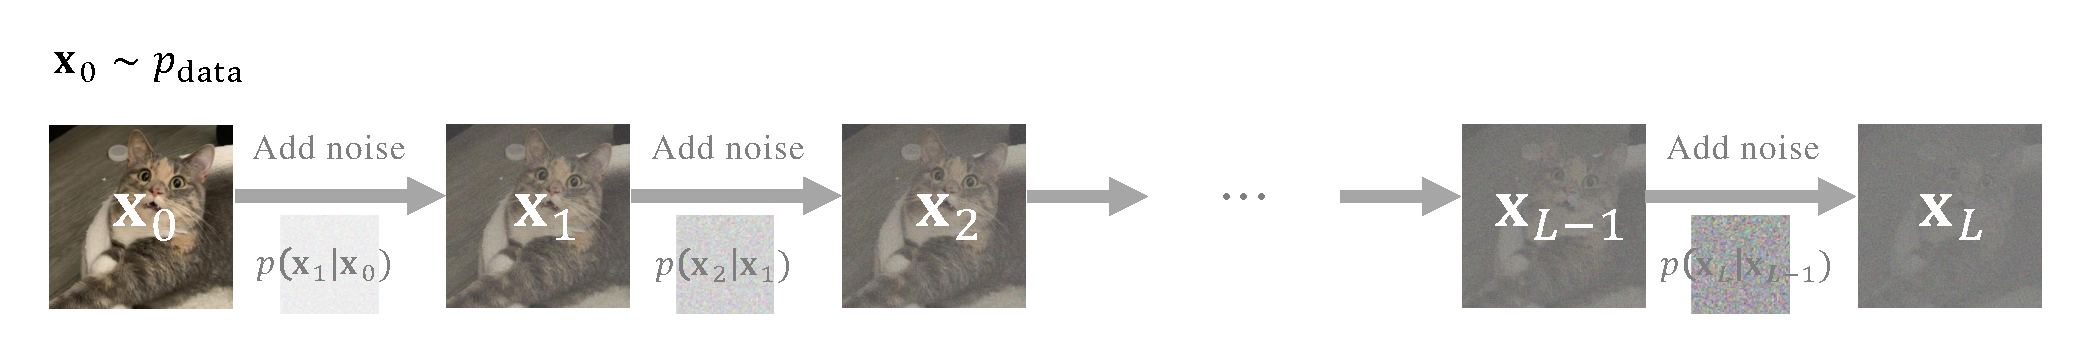
\includegraphics[width=\linewidth]{Images/PartB/vdm-forward.pdf}
    \caption{DDPM 前向过程的示意图，其中高斯噪声被逐步添加，将一个数据样本腐蚀为纯噪声。\figcredit{由作者绘制。}}
    \label{fig:vdm-forward}
\end{figure}

% \se{check indexing ranges below (from 0 or 1), seems off by one}

让我们将这种逐步退化形式化：
\paragraph{固定的高斯转移。}
前向过程中的每一步由一个固定的高斯转移核\footnote{这一表述虽然在形式上可能看起来不同，但在数学上等价于原始的 DDPM 转移核。}控制：
\[
p(\rvx_i|\rvx_{i-1}) := \mathcal{N}(\rvx_i; \sqrt{1 - \beta_i^2}   \rvx_{i-1}, \beta_i^2 \rmI).
\]
这里，过程从 $\rvx_{0} $ 开始，表示从真实数据分布 $p_{\text{data}}$ 中抽取的一个样本。序列 $\{\beta_i\}_{i=1}^L$ 表示一个预先确定的、单调递增的噪声调度，其中每个
$\beta_i \in (0, 1)$ 控制第 $i$ 步注入的高斯噪声的方差。为方便起见，我们定义 $\alpha_i := \sqrt{1 - \beta_i^2}$。这一定义与如下直观的迭代更新精确等价：
\[
\rvx_i = \alpha_i \rvx_{i-1} + \beta_i \bm{\epsilon}_i,  
\]
其中 $\bm{\epsilon}_i \sim \mathcal{N}(\bm{0}, \rmI)$ 是独立同分布的。这意味着在每一步 $i$，我们将前一状态 $\rvx_{i-1}$ 按 $\alpha_i$ 缩小，并添加一个由 $\beta_i$ 缩放的控制量的高斯噪声。

\paragraph{扰动核与先验分布。}
通过递归地应用转移核，我们得到了给定原始数据 $\rvx_0$ 时第 $i$ 步噪声样本分布的闭式表达式：
\[
p_i(\rvx_i|\rvx_0) = \mathcal{N}\left(\rvx_i; \bar{\alpha}_i \rvx_0, (1 - \bar{\alpha}_i^2) \rmI \right),
\]
其中
\[
\bar{\alpha}_i := \prod_{k=1}^i \sqrt{1-\beta_k^2} = \prod_{k=1}^i \alpha_k.
\]
这意味着我们可以直接从 $\rvx$ 采样 $\rvx_i$，如
\begin{align}\label{eq:ddpm-forward}
    \rvx_i = \bar{\alpha}_i \rvx_0 + \sqrt{1-\bar{\alpha}_i^2}   \bm{\epsilon}, \quad \bm{\epsilon} \sim \mathcal{N}(\bm{0}, \rmI).
\end{align}
令噪声调度 $ \{\beta_i\}_{i=1}^L $ 为一个递增序列，则前向过程的边际分布收敛为
\[
p_L(\mathbf{x}_L | \rvx_0) \longrightarrow \mathcal{N}(\mathbf{0}, \mathbf{I}) \quad \text{as } L \to \infty,
\]
这激发了对先验分布的选择
\[
p_{\text{prior}} := \mathcal{N}(\mathbf{0}, \mathbf{I})
\]
且不依赖于数据 $\rvx_0$。
% \paragraph{Marginal Densities.}
% By marginalizing over the data distribution using the law of total probability, the marginal density at step $i$ is
% \[
% p_i(\rvx_i) := \int p_i(\rvx_i|\rvx) p_{\text{data}}(\rvx_0) \diff \rvx_0.
% \]
% \se{what's the point of this paragraph?}


\subsection{反向去噪过程（可学习的解码器）}

% \se{this section packs too much content, too many formulas and will be overwhelming. since it is important, you need to break it up more and more gradually} \jcc{I cut the original section into 3 subsections: one is about oracle $p(\rvx_{i-1}|\rvx_i)$ and introduce high-level idea; the next subsection is about how to model $p_\bphi(\rvx_{i-1}|\rvx_i)$ with practical losses/parametrizations introduced there (\S 2.2.3); and the last one is Practical Choices of Predictions and Loss (\S 2.2.4). Also, I added some bridging and intuition.}

DDPM 的核心本质在于其\emph{反转}前向扩散过程所施加的受控退化的能力。从纯的、无结构的噪声 $\mathbf{x}_L \sim p_{\text{prior}}$ 出发，目标是逐步\emph{去噪}这种随机性，一步接一步，直到一个连贯而有意义的数据样本出现。这一反向生成通过一条马尔可夫链进行，如 \Cref{fig:ddpm-sampling-formal-rev} 所示。
\begin{figure}[tbh!]
    \centering
    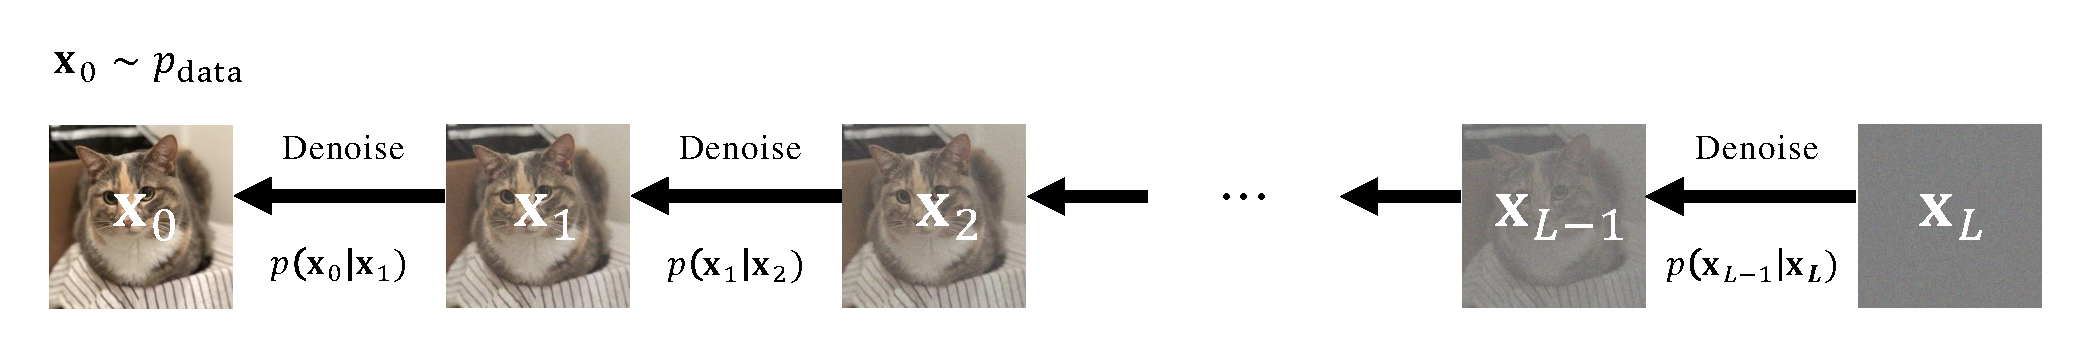
\includegraphics[width=\linewidth]{Images/PartB/vdm-backward.pdf}
\caption{\textbfs{DDPM 反向（去噪）过程示意图。}从噪声 $\mathbf{x}_L \sim  p_{\mathrm{prior}}$ 出发，模型依次采样 $\mathbf{x}_{i-1} \sim  p(\mathbf{x}_{i-1}|\mathbf{x}_i)$（$i=L,\ldots,1$）以获得新生成的数据 $\mathbf{x}_0$。先验的转移 $p(\mathbf{x}_{i-1}|\mathbf{x}_i)$ 是未知的；因此，我们的目标是近似它。
\figcredit{由作者绘制。}
}

    \label{fig:ddpm-sampling-formal-rev}
\end{figure}





那么，指导 DDPM 发展的根本挑战和核心问题就变成：
\begin{question}
我们能否精确计算，或至少有效地近似这些反向转移核 $ p(\mathbf{x}_{i-1}|\mathbf{x}_i) $，尤其是在考虑 $\mathbf{x}_i \sim p_i(\mathbf{x}_i)$ 的复杂分布时？
\end{question}

我们不立即深入证据下界（ELBO）的数学上错综复杂的推导（正如原始 DDPM 论文所做的，其详细讨论留待 \Cref{subsec:ddpm-elbo}），而是从一个更直观的视角来处理训练目标：利用条件概率来获得一个可处理的表述。


\paragraph{概述：建模与训练目标。} 
为了实现生成过程，我们的目标是近似未知的真实反向转移核 $p(\mathbf{x}_{i-1}|\mathbf{x}_i)$。我们通过引入一个可学习的参数化模型 $p_{\bm{\phi}}(\mathbf{x}_{i-1}|\mathbf{x}_i)$，并训练它以最小化期望 KL 散度来实现这一点：
\begin{align}\label{eq:marginal-kl-matching}
    \mathbb{E}_{p_i(\mathbf{x}_i)} \left[
    \mathcal{D}_{\mathrm{KL}}\big(p(\mathbf{x}_{i-1}|\mathbf{x}_i) \| p_{\bm{\phi}}(\mathbf{x}_{i-1}|\mathbf{x}_i)\big)
    \right].
\end{align}

然而，对目标分布 $p(\mathbf{x}_{i-1}|\mathbf{x}_i)$ 的直接计算具有挑战性。由贝叶斯定理，我们需要计算：
\[
p(\mathbf{x}_{i-1}|\mathbf{x}_i) = p(\mathbf{x}_i|\mathbf{x}_{i-1}) \underbrace{\frac{p_{i-1}(\mathbf{x}_{i-1})}{p_i(\mathbf{x}_i)}}_{\text{intractable}}.
\]
边际分布 $p_i(\rvx_i)$ 和 $p_{i-1}(\rvx_{i-1})$ 是对未知数据分布 $p_{\mathrm{data}}$ 的期望，由下式给出：
\[
p_i(\rvx_i) = \int p_i(\rvx_i | \rvx_0) p_{\mathrm{data}}(\rvx_0) \mathrm{d}\rvx_0,
\]
$p_{i-1}(\rvx_{i-1})$ 类似。由于 $p_{\mathrm{data}}$ 未知，这些积分没有闭式求值；充其量只能用样本来近似，因此实践中无法得到精确的密度。

\begin{figure}[th!]
    \centering
    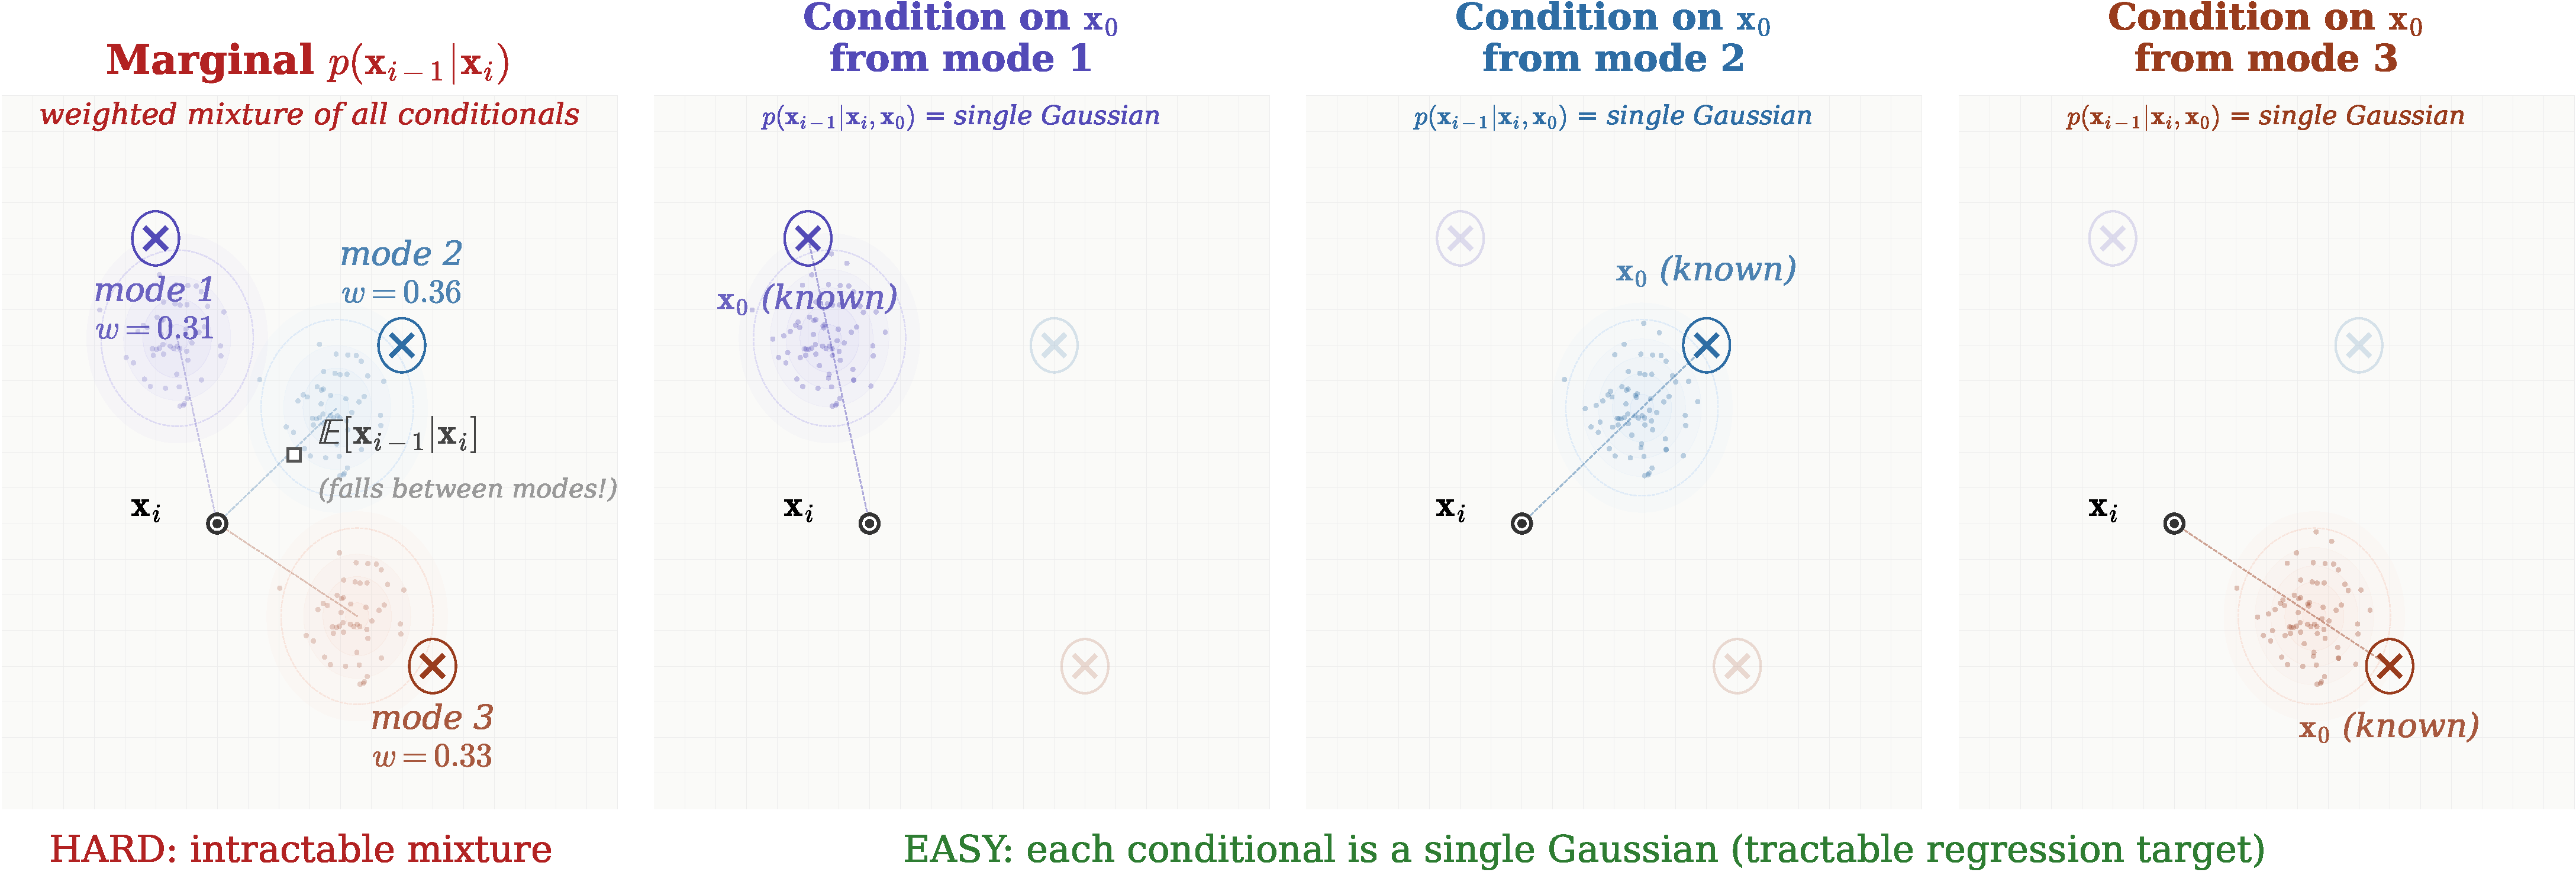
\includegraphics[width=\linewidth]{Images/PartB/ddpm_conditional_trick.pdf}
    \caption{\textbfs{DDPM 中条件化技巧的示意图。}
对于一个固定的噪声样本 $\rvx_i$，真实的反向分布
$p(\rvx_{i-1}|\rvx_i)$ 是通过对所有可能的干净来源 $\rvx_0$ 边际化诱导的，因此通常是一个可能是多峰的混合分布。
它的均值甚至可能落在模式之间，使得直接预测变得困难。
相比之下，一旦我们对干净样本 $\rvx_0$ 进行条件化，反向后验
$p(\rvx_{i-1}|\rvx_i,\rvx_0)$ 就变成单个高斯分布。
DDPM 在训练中利用了这一可处理的条件结构，用一个可处理的回归目标代替了困难的多峰预测问题。\figcredit{由作者在 AI 辅助编程下绘制。}}
    \label{fig:conditional-trick}
\end{figure}


\paragraph{用条件化克服不可处理性。}
DDPM 中的一个核心洞察解决了这一不可处理性：我们用干净的数据样本 $\mathbf{x}_0$ 对反向转移进行条件化。这一微妙却有力的步骤将不可处理的核转化为一个数学上可处理的核：
\[
p(\mathbf{x}_{i-1}|\mathbf{x}_i, \mathbf{x}_0) = p(\mathbf{x}_i|\mathbf{x}_{i-1}) \frac{p(\mathbf{x}_{i-1}|\mathbf{x}_0)}{p(\mathbf{x}_i|\mathbf{x}_0)}.
\]
这一可处理性源于前向过程的两个关键性质：其马尔可夫性质，即 $p(\mathbf{x}_i|\mathbf{x}_{i-1}, \mathbf{x}_0) = p(\mathbf{x}_i|\mathbf{x}_{i-1})$，以及所有相关分布的高斯性质。因此，$p(\mathbf{x}_{i-1}|\mathbf{x}_i, \mathbf{x}_0)$ 本身是高斯的，并具有闭式表达式（我们将在 \Cref{eq:ddpm-reverse-mean} 中看到）。我们在 \Cref{fig:conditional-trick} 中对其进行了可视化。关键的是，这种优雅的条件化策略使我们能够推导出一个可处理的目标，它在功能上等价于 \Cref{eq:marginal-kl-matching} 中看似不可处理的边际 KL 散度。

\thmp{边际 KL 与条件 KL 最小化的等价性}{equiv-marginal-kl}{
如下等式成立：
\begin{align}\label{eq:kl-matching}
\begin{aligned}
    &\mathbb{E}_{p_i(\rvx_i)}\left[
        \mathcal{D}_{\mathrm{KL}}\big(p(\rvx_{i-1}|\rvx_i) \| p_{\bm{\phi}}(\rvx_{i-1}|\rvx_i)\big)
    \right] \\
    ={}&
    \mathbb{E}_{p_{\mathrm{data}}(\rvx_0)}
    \mathbb{E}_{p(\rvx_i|\rvx_0)} \left[
        \mathcal{D}_{\mathrm{KL}}\big(p(\rvx_{i-1}|\rvx_i, \rvx_0) \| p_{\bm{\phi}}(\rvx_{i-1}|\rvx_i)\big)
    \right] + C.
\end{aligned}
\end{align}
其中 $C$ 是与 $\bm{\phi}$ 无关的常数。此外，\Cref{eq:kl-matching} 的最小化子满足
\[
p^*(\mathbf{x}_{i-1}|\mathbf{x}_i) = \mathbb{E}_{p(\mathbf{x}_0|\mathbf{x}_i)} \big[p(\mathbf{x}_{i-1}|\mathbf{x}_i, \mathbf{x}_0)\big] = p(\mathbf{x}_{i-1}|\mathbf{x}_i), \quad \mathbf{x}_i \sim p_i.
\]
}{证明通过展开定义、应用概率的链式法则，并利用一个对数恒等式，将一个 KL 散度期望重写为一个期望条件 KL 散度与一个边际 KL 散度之和。完整的推导见 \Cref{subsec:proof-equiv-marginal-kl}。}


这一替代视角——通过条件化获得一个可处理的目标——构成了 DDPM 的基础，并揭示了与其他有影响力的扩散模型的深刻共性，正如我们将在 \Cref{ch:score-based} 和 \Cref{ch:flow-based} 中探讨的那样。


它揭示了一个有力的等价性：最小化边际分布之间的 KL 散度在数学上等价于最小化特定条件分布之间的 KL 散度。后一种表述异常有用，因为关键的条件分布 $p(\mathbf{x}_{i-1}|\mathbf{x}_i, \mathbf{x})$ 具有一个方便的闭式表达式：
\lem{反向条件转移核}{ddpm-reverse-kernel}{$p(\mathbf{x}_{i-1} | \mathbf{x}_i, \mathbf{x})$ 是高斯分布，具有如下闭式表达式：
\begin{align*}
    p(\rvx_{i-1} | \rvx_i, \rvx) =\mathcal{N}\left(\rvx_{i-1}; \bm{\mu}\left(\rvx_i, \rvx, i\right), \sigma^2(i)\rmI \right),
\end{align*}
其中
\begin{align}\label{eq:ddpm-reverse-mean}
\begin{aligned}
            \bm{\mu}\left(\rvx_i, \rvx, i\right):= \frac{\bar{\alpha}_{i-1}\beta_i^2}{1-\bar{\alpha}_i^2}\rvx + \frac{(1-\bar{\alpha}_{i-1}^2)\alpha_i }{1-\bar{\alpha}_i^2}\rvx_i,
\quad  \sigma^2(i) := \frac{1-\bar{\alpha}_{i-1}^2}{1-\bar{\alpha}_i^2}\beta_i^2.
\end{aligned}
\end{align}
}
在后面的引理~\ref{reverse-kernel} 中，我们给出了一个更通用的公式，它超越了 \Cref{eq:ddpm-forward} 中描述的 DDPM 加噪过程。


\subsection{反向转移核 $p_{\bm{\phi}}(\mathbf{x}_{i-1}|\mathbf{x}_i)$ 的建模} 利用定理~\ref{thm:equiv-marginal-kl} 中梯度层面的等价性以及引理~\ref{ddpm-reverse-kernel} 中反向条件 $p(\mathbf{x}_{i-1}|\mathbf{x}_i, \mathbf{x})$ 的高斯形式，DDPM 假设每个反向转移 $p_{\bm{\phi}}(\rvx_{i-1}| \rvx_i)$ 是高斯的，参数化为
\begin{align}\label{eq:def-reverse}
    p_{\bm{\phi}}(\mathbf{x}_{i-1}|\mathbf{x}_i) := \mathcal{N}\big(\mathbf{x}_{i-1}; \bm{\mu}_{\bm{\phi}}(\mathbf{x}_i, i), \sigma^2(i) \mathbf{I}\big),
\end{align}
其中 $\bm{\mu}_{\bm{\phi}}(\cdot, i) \colon \mathbb{R}^D \to \mathbb{R}^D$ 是一个可学习的均值函数，$\sigma^2(i) > 0$ 固定为 \Cref{eq:ddpm-reverse-mean} 中所定义。

我们将时间步 $i$ 上取平均、以数据 $\rvx_0 \sim p_{\text{data}}$ 为条件的 KL 散度记为匹配所有层分布：
\begin{align}\label{eq:ddpm-diffusion}
    \mathcal{L}_{\text{diffusion}}(\rvx_0;\bm{\phi}) := \sum_{i=2}^L \mathbb{E}_{p(\rvx_i|\rvx_0)}\left[\mathcal{D}_{\text{KL}}\big(p(\rvx_{i-1}|\rvx_i, \rvx_0)  \Vert  p_{\bm{\phi}}(\rvx_{i-1}|\rvx_i)\big)\right].
\end{align}
由于两个分布都是高斯的，且采用 \Cref{eq:def-reverse} 中定义的参数化，该目标具有闭式表达式，并可简化为：
\begin{align}\label{eq:ddpm-diffusion-simp}
    \mathcal{L}_{\text{diffusion}}(\rvx_0;\bm{\phi}) = \sum_{i=2}^L \frac{1}{2\sigma^2(i)}  \mathbb{E}_{p(\rvx_i|\rvx_0)}\left\| \bm{\mu}_{\bm{\phi}}(\rvx_i, i) - \bm{\mu}(\rvx_i, \rvx_0, i) \right\|_2^2 + C,
\end{align}
其中 $C$ 是与 $\bm{\phi}$ 无关的常数。对数据分布取平均并省略常数 $C$（它不影响优化），最终的 DDPM 训练目标为
\begin{align}
\begin{aligned}
    \label{eq:ddpm-mean-loss}
    \mathcal{L}_{\text{DDPM}}(\bm{\phi}) := \sum_{i=2}^L \frac{1}{2\sigma^2(i)}  \mathbb{E}_{\rvx_0} \mathbb{E}_{p(\mathbf{x}_i|\rvx_0)} \left[ \left\| \bm{\mu}_{\bm{\phi}}(\mathbf{x}_i, i) - \bm{\mu}(\mathbf{x}_i, \rvx_0, i) \right\|_2^2 \right],
\end{aligned}
\end{align}
其中 $\rvx_0\sim p_{\mathrm{data}}$。

\subsection{预测与损失的实际选择}\label{subsec:ddpm-prediction}

\paragraph{$\beps$-预测。}
在典型的 DDPM 实现中，训练并不直接使用 \Cref{eq:ddpm-mean-loss} 中基于\emph{均值预测}参数化的原始损失。相反，通常采用一种等价的重参数化，即\emph{$\beps$-预测}（噪声预测）形式。

回想在 DDPM 前向过程中，噪声水平 $i$ 处的一个噪声样本 $\rvx_i \sim p(\rvx_i |\rvx_0)$ 通过下式生成
\begin{equation}\label{eq:ddpm-perturbation}
    \rvx_i = \bar{\alpha}_i \rvx_0 + \sqrt{1 - \bar{\alpha}_i^2}   \boldsymbol{\epsilon}, \quad \rvx_0 \sim p_{\text{data}}, \quad \boldsymbol{\epsilon} \sim \mathcal{N}(\mathbf{0}, \mathbf{I}).
\end{equation}
利用这一表达式，\Cref{eq:ddpm-reverse-mean} 中的反向均值 $\bm{\mu}(\rvx_i, \rvx_0, i)$ 可以重写为：
\[
\bm{\mu}(\rvx_i, \rvx_0, i) = \frac{1}{\alpha_i} \left( \rvx_i - \frac{1 - \alpha_i^2}{\sqrt{1 - \bar{\alpha}_i^2}} \boldsymbol{\epsilon} \right).
\]

这激发了对模型均值 $\bm{\mu}_{\bm{\phi}}$ 的一种参数化，使用一个直接预测噪声的神经网络 $\boldsymbol{\epsilon}_{\bm{\phi}}(\rvx_i, i)$：
\[
\bm{\mu}_{\bm{\phi}}(\rvx_i, i) = \frac{1}{\alpha_i} \left( \rvx_i - \frac{1 - \alpha_i^2}{\sqrt{1 - \bar{\alpha}_i^2}} \underbrace{\boldsymbol{\epsilon}_{\bm{\phi}}(\rvx_i, i)}_{\beps\text{-prediction}} \right).
\]
将其代入原始损失，得到预测噪声与真实噪声之间的一个平方 $\ell_2$ 误差：
\[
\left\| \bm{\mu}_{\bm{\phi}}(\rvx_i, i) - \bm{\mu}(\rvx_i, \rvx_0, i) \right\|_2^2 \propto \left\| \boldsymbol{\epsilon}_{\bm{\phi}}(\rvx_i, i) - \boldsymbol{\epsilon} \right\|_2^2,
\]
至多差一个依赖于 $i$ 的加权因子。直观地说，模型扮演“噪声侦探”的角色，估计前向过程中每一步添加的随机噪声。从被腐蚀的样本中减去这一估计，会使其更接近干净的原始样本，而一步一步地重复这一过程就从纯噪声中重建出数据。

\paragraph{带有 $\beps$-预测的简化损失。}
在实践中，这一表达式通过省略加权项被进一步简化，得到广泛使用的 DDPM 训练损失：
\begin{equation}\label{eq:ddpm-simple-loss}
    \mathcal{L}_{\text{simple}}(\bm{\phi}) := \mathbb{E}_{i} \mathbb{E}_{\rvx \sim p_{\text{data}}(\rvx)} \mathbb{E}_{\boldsymbol{\epsilon} \sim \mathcal{N}(\mathbf{0}, \mathbf{I})} \left[ \left\| \boldsymbol{\epsilon}_{\bm{\phi}}(\rvx_i, i) - \boldsymbol{\epsilon} \right\|_2^2 \right],
\end{equation}
其中 $\rvx_i = \bar{\alpha}_i \rvx_0 + \sqrt{1 - \bar{\alpha}_i^2} \boldsymbol{\epsilon}$，$\rvx_0 \sim p_{\text{data}}$。由于目标噪声在每个时间步 $t$ 都具有单位方差，\Cref{eq:ddpm-simple-loss} 中的 $\ell_2$ 损失在所有 $t$ 上保持一致的尺度。这防止了目标的消失或爆炸，并消除了显式损失加权的需要。


重要的是，$\mathcal{L}_{\text{DDPM}}$ 和 $\mathcal{L}_{\text{simple}}$ 共享相同的最优解 $\boldsymbol{\epsilon}^*$，这是因为 \Cref{eq:ddpm-simple-loss} 本质上退化为一个最小二乘问题（类似地如命题~\ref{dsm-minimizer} 或命题~\ref{equi-para} 所示）：
\[
\boldsymbol{\epsilon}^*(\rvx_i, i) = \mathbb{E}\left[ \boldsymbol{\epsilon}|\rvx_i \right], \quad \rvx_i \sim p_i.
\]
直观地说，$\beps$-预测网络 $\boldsymbol{\epsilon}_{\bm{\phi}}(\rvx_i, i)$ 估计前向过程为产生 $\rvx_i$ 而添加的噪声。在最优时，这一估计与真实噪声的条件期望一致，尽管 $\rvx_i$ 并不唯一地确定原始干净样本。

\paragraph{另一种等价的参数化：$\rvx$-预测。}
\Cref{eq:ddpm-reverse-mean} 启发了一种替代但等价的参数化，称为\emph{$\rvx$-预测}（干净预测），其中一个神经网络 $\rvx_{\bm{\phi}}(\rvx_i, i)$ 被训练以从给定的噪声输入 $\rvx_i \sim p_i(\rvx_i)$ 在噪声水平 $i$ 处预测一个干净（去噪）样本。将反向均值表达式中的真实干净样本 $\rvx_0$ 替换为 $\rvx_{\bm{\phi}}(\rvx_i, i)$ 得到如下模型：
\begin{align*}
\bm{\mu}_{\bm{\phi}}(\rvx_i, i) = \frac{\bar{\alpha}_{i-1} \beta_i^2}{1 - \bar{\alpha}_i^2} \rvx_{\bm{\phi}}(\rvx_i, i) + \frac{(1 - \bar{\alpha}_{i-1}^2)\alpha_i}{1 - \bar{\alpha}_i^2} \rvx_i.
\end{align*}
类似于 $\beps$-预测形式，训练目标可以表示为
\[
\left\| \bm{\mu}_{\bm{\phi}}(\rvx_i, i) - \bm{\mu}(\rvx_i, \rvx_0, i) \right\|_2^2 \propto \left\| \rvx_{\bm{\phi}}(\rvx_i, i) - \rvx_0 \right\|_2^2, \quad \rvx_0 \sim p_{\text{data}},
\]
其中模型被训练以从其噪声版本 $\rvx_i$ 预测原始数据样本 $\rvx_0$。这一等价性将 \Cref{eq:ddpm-mean-loss} 中的均值匹配损失简化为
\[
\mathbb{E}_{i} \mathbb{E}_{\rvx_0 \sim p_{\text{data}}} \mathbb{E}_{\boldsymbol{\epsilon} \sim \mathcal{N}(\mathbf{0}, \mathbf{I})} \left[\omega_i \left\| \rvx_{\bm{\phi}}(\rvx_i, i) - \rvx_0 \right\|_2^2 \right],
\]
对某个加权函数 $\omega_i$。由于这是一个最小二乘问题，最优解由（见命题~\ref{dsm-minimizer} 或命题~\ref{equi-para}）
\begin{align}\label{eq:ddpm-clean-minimizer}
    \rvx^*(\rvx_i, i) = \mathbb{E}\left[ \rvx_0|\rvx_i \right], \quad \rvx_i \sim p_i,
\end{align}
给出，即模型应在时间步 $i$ 给定噪声观测 $\rvx_i$ 时预测期望的干净数据。

$\rvx$-预测和 $\beps$-预测参数化在数学上是等价的，并通过前向过程联系起来：
\begin{equation}\label{eq:ddpm-clean-noise}
    \rvx_i = \bar{\alpha}_i \rvx_{\bm{\phi}}(\rvx_i, i) + \sqrt{1 - \bar{\alpha}_i^2}   \boldsymbol{\epsilon}_{\bm{\phi}}(\rvx_i, i).
\end{equation}
也就是说，人们既可以预测干净样本 $\rvx_{\bm{\phi}}(\rvx_i, i)$，也可以预测噪声 $\boldsymbol{\epsilon}_{\bm{\phi}}(\rvx_i, i)$，使得它们的组合在前向加噪过程下重现 $\rvx_i$。 




\subsection{DDPM 的 ELBO}\label{subsec:ddpm-elbo} 将反向转移如 \Cref{eq:def-reverse} 中那样定义后，这导出了 DDPM 中联合生成分布的定义：
\[
p_{\bm{\phi}}(\rvx_0, \rvx_{1:L}) := p_{\bm{\phi}}(\rvx_0|\rvx_1)  p_{\bm{\phi}}(\rvx_1|\rvx_2)\cdots p_{\bm{\phi}}(\rvx_{L-1}|\rvx_L)   p_{\text{prior}}(\rvx_L),
\]
而数据的边际生成模型由下式给出：
\begin{align*}
    p_{\bm{\phi}}(\rvx_0) := \int p_{\bm{\phi}}(\rvx_0, \rvx_{1:L}) \diff \rvx_{1:L}.
\end{align*}

事实上，通过 \Cref{eq:ddpm-diffusion} 进行的 DDPM 训练可以严格地建立在极大似然估计（\Cref{eq:MLE}）之上。具体而言，其目标构成一个 ELBO，类似于 \Cref{sec:vae} 中 VAE 和 HVAE 的 ELBO，它作为对数密度的下界：
\thmp{DDPM 的 ELBO}{ddpm-elbo}{    
\begin{align}\label{eq:ddpm-elbo}
        \begin{aligned}
        -\log p_{\bm{\phi}}(\rvx_0)  &\leq-\mathcal{L}_{\text{ELBO}}(\rvx_0; \bm{\phi}) 
        \\&:= \mathcal{L}_{\text{prior}}(\rvx_0) + \mathcal{L}_{\text{recon.}}(\rvx_0;\bm{\phi})  + \mathcal{L}_{\text{diffusion}}(\rvx_0;\bm{\phi})
        \end{aligned}
\end{align}
这里，损失的每个分量定义为：
\begin{align*}
   \mathcal{L}_{\text{prior}}(\rvx_0) &:= \mathcal{D}_{\text{KL}}\Big( p(\rvx_L|\rvx_0) \Vert p_{\text{prior}}(\rvx_L)\Big)\\
   \mathcal{L}_{\text{recon.}}(\rvx_0;\bm{\phi}) &:= \mathbb{E}_{p(\rvx_1|\rvx_0)}\left[-\log p_{\bm{\phi}}(\rvx_0|\rvx_1)\right]\\
   \mathcal{L}_{\text{diffusion}}(\rvx_0;\bm{\phi}) &= \sum_{i=2}^L  \mathbb{E}_{p(\rvx_i|\rvx_0)}\left[\mathcal{D}_{\text{KL}}\Big(p(\rvx_{i-1}|\rvx_i, \rvx_0) \Vert p_{\bm{\phi}}(\rvx_{i-1}|\rvx_i) \Big)\right]. 
\end{align*}}{该推导应用了 Jensen 不等式，如同 HVAE/VAE 的 ELBO（\Cref{eq:hvae-elbo}），并作了进一步简化。详细证明留待 \Cref{app:vlb-proof}。
}
ELBO $\mathcal{L}_{\text{ELBO}}$ 由三项组成：
\begin{itemize}
    \item $\mathcal{L}_{\text{prior}}$ 可以通过选择噪声调度 $\{\beta_i\}$ 使得 $p(\cdot|\rvx_0) \approx p_{\text{prior}}(\cdot)$ 而变得可忽略。
    \item 对于 $\mathcal{L}_{\text{recon.}}$，可以用蒙特卡洛估计来近似和优化；实际实现见 \citep{ho2020denoising, kingma2021variational}。
    \item $\mathcal{L}_{\text{diffusion}}$（参见 \Cref{eq:ddpm-diffusion}）在所有步骤 $i$ 上将反向条件分布 $p_{\bm{\phi}}(\mathbf{x}_{i-1}|\mathbf{x}_i)$ 匹配到 $p(\mathbf{x}_{i-1}|\mathbf{x}_i)$。
\end{itemize}

ELBO 目标 $\mathcal{L}_{\text{ELBO}}$ 也可以通过带有隐变量 $\rvz = \rvx_{1:L}$ 的数据处理不等式视角来解释，如 \Cref{eq:joint-bound} 所示：
\begin{align*}
    \mathcal{D}_{\mathrm{KL}}(p_{\mathrm{data}}(\rvx_0) \| p_{\bm{\phi}}(\rvx_0)) \leq \mathcal{D}_{\mathrm{KL}}\left(p(\rvx_0, \rvx_{1:L}) \| p_{\bm{\phi}}(\rvx_0, \rvx_{1:L})\right),
\end{align*}
其中 $p(\rvx_0, \rvx_{1:L}) := p_{\mathrm{data}}(\rvx_0)  p(\rvx_1|\rvx_0)  p(\rvx_2|\rvx_1) \cdots p(\rvx_L|\rvx_{L-1})$ 表示沿前向过程的联合分布。 




\rmkb{扩散模型的变分视角契合 HVAE 模板：“编码器”是固定的前向加噪链，隐变量 $\mathbf{x}_{1:T}$ 与数据共享维度。训练最大化同一个 ELBO。这里没有学习得到的编码器，也没有逐层的 KL 项；相反，目标分解为从大到小噪声（由粗到细）的良好条件化的去噪子问题，从而产生稳定的优化和较高的样本质量，同时沿时间/噪声保留了一个由粗到细的层次。
 }





\subsection{采样}
在训练好 $\beps$-预测模型 $\bm{\epsilon}_{\bm{\phi}^\times}(\rvx_i, i)$\footnote{我们使用符号“$\times$”来表示模型已经训练完毕且现在被冻结。}之后，采样如 \Cref{fig:ddpm-sampling-formal-rev} 所示顺序进行，使用参数化的转移 $p_{\bm{\phi}^\times}(\rvx_{i-1} | \rvx_i)$。


更具体地说，从一个随机种子 $\rvx_L \sim p_{\text{prior}} = \mathcal{N}(\bm{0},\rmI)$ 出发，我们对 $i = L, L-1, \dots, 1$ 按照如下更新规则从 $p_{\bm{\phi}^\times}(\rvx_{i-1} | \rvx_i)$ 递归地采样：
\begin{align}\label{eq:ddpm-sampling}
    \rvx_{i-1} \leftarrow \underbrace{\frac{1}{\alpha_i}\left( \rvx_i  - \frac{1-\alpha_i^2}{\sqrt{1-\bar{\alpha}_i^2}} \bm{\epsilon}_{\bm{\phi}^\times}(\rvx_i, i)\right)}_{\bm{\mu}_{\bm{\phi}^\times}(\rvx_i, i)} +\sigma(i) \bm{\epsilon}_i,\quad \bm{\epsilon}_i\sim  \mathcal{N}(\bm{0},\rmI).
\end{align}
这一“去噪”过程持续进行，直到获得 $\rvx_0$ 作为最终的干净生成样本。 



% \paragraph{Another Interpretation of DDPM's Sampling.} From \Cref{eq:ddpm-clean-noise}, the clean sample prediction corresponding to a noise estimate $\boldsymbol{\epsilon}_{\bm{\phi}^\times}(\rvx_i, i)$ can be expressed as
% \[
% \rvx_{\bm{\phi}^\times}(\rvx_i, i) = \frac{\rvx_i - \sqrt{1 - \bar{\alpha}_i^2}   \boldsymbol{\epsilon}_{\bm{\phi}^\times}(\rvx_i, i)}{\bar{\alpha}_i}.
% \]
% Plugging this into the DDPM sampling rule in \Cref{eq:ddpm-sampling} yields the equivalent update:
% \[
% \rvx_{i-1} \leftarrow \text{(interpolation between $\rvx_i$ and clean prediction $\rvx_{\bm{\phi}^\times}$)} + \sigma(i) \boldsymbol{\epsilon}_i
% \]
% indicating that each step is centered around the predicted clean sample, with added Gaussian noise scaled by $\sigma(i)$.

% \paragraph{Another Interpretation of DDPM Sampling.}
% A useful way to interpret DDPM sampling is to rewrite the predicted noise in terms of the current sample $\rvx_i$ and the predicted clean sample $\rvx_{\bm{\phi}^\times}(\rvx_i,i)$. From \Cref{eq:ddpm-clean-noise},
% \[
% \boldsymbol{\epsilon}_{\bm{\phi}^\times}(\rvx_i,i)
% =
% \frac{\rvx_i-\bar{\alpha}_i\,\rvx_{\bm{\phi}^\times}(\rvx_i,i)}{\sqrt{1-\bar{\alpha}_i^2}}.
% \]
% Substituting this expression into the DDPM sampling rule in \Cref{eq:ddpm-sampling} gives
% \[
% \rvx_{i-1}
% \leftarrow
% \underset{\text{interpolation between $\rvx_i$ and clean prediction $\rvx_{\bm{\phi}^\times}$}}{\underbrace{\frac{\alpha_i(1-\bar{\alpha}_{i-1}^2)}{1-\bar{\alpha}_i^2}\,\rvx_i
% +
% \frac{\bar{\alpha}_{i-1}\beta_i^2}{1-\bar{\alpha}_i^2}\,\rvx_{\bm{\phi}^\times}(\rvx_i,i)
% }}
% +
% \sigma(i)\,\boldsymbol{\epsilon}_i.
% \]
% Thus, the mean of the DDPM update is an interpolation between the current noisy sample $\rvx_i$ and the predicted clean sample $\rvx_{\bm{\phi}^\times}(\rvx_i,i)$, followed by Gaussian perturbation with scale $\sigma(i)$.

% This reveals that DDPM sampling can be viewed as an iterative denoising process that alternates between:
% \begin{enumerate}
%     \item Estimating the clean data $\mathbf{x}_{\bm{\phi}^\times}(\mathbf{x}_i, i)$ from the current noisy input $\mathbf{x}_i$,
%     \item Sampling a less noisy latent $\mathbf{x}_{i-1}$ via the update rule using this clean estimate.
% \end{enumerate}



% However, even if $\mathbf{x}_{\bm{\phi}^\times}$ is trained as the optimal denoiser (i.e., the conditional expectation minimizer; see \Cref{eq:ddpm-clean-minimizer}), it can only predict the \emph{average} clean sample given $\rvx_i$. This limitation leads to blurry predictions, particularly at high noise levels, where recovering detailed structure from severely corrupted inputs becomes difficult.


% From this viewpoint, diffusion sampling typically moves from high to low noise and progressively refines an estimate of the clean signal. Early steps set the global structure, later steps add fine detail, and the sample becomes more realistic as the noise is removed.


\paragraph{DDPM 采样的另一种解释。}

解释 DDPM 采样的一种有用方式是重写更新规则
使噪声水平的结构变得显式。
回想 \Cref{eq:ddpm-clean-noise}，预测噪声可以用
当前样本 $\rvx_i$ 和预测的
干净样本 $\rvx_{\bm{\phi}^\times}(\rvx_i,i)$ 表示为：
\[
\boldsymbol{\epsilon}_{\bm{\phi}^\times}(\rvx_i,i)
=
\frac{\rvx_i - \bar{\alpha}_i\,\rvx_{\bm{\phi}^\times}(\rvx_i,i)}
     {\sqrt{1-\bar{\alpha}_i^2}}.
\]
将其代入 DDPM 采样规则
（\Cref{eq:ddpm-sampling}）并整理，我们得到
\begin{equation}\label{eq:ddpm-renoise}
\rvx_{i-1}
\;\leftarrow\;
\bar{\alpha}_{i-1}\,\rvx_{\bm{\phi}^\times}(\rvx_i,i)
\;+\;
\underbrace{
  \sqrt{1-\bar{\alpha}_{i-1}^2 - \tilde{\beta}_i^2}\;
  \boldsymbol{\epsilon}_{\bm{\phi}^\times}(\rvx_i,i)
  \;+\;
  \tilde{\beta}_i\,\boldsymbol{\epsilon}_i
}_{\text{combined std.\ }=\;\sqrt{1-\bar{\alpha}_{i-1}^2}},
\end{equation}
其中 $\tilde{\beta}_i^2
= \frac{(1-\bar{\alpha}_{i-1}^2)(1-\alpha_i^2)}{1-\bar{\alpha}_i^2}$
是 DDPM 后验方差\footnote{%
系数
$\sqrt{1-\bar{\alpha}_{i-1}^2 - \tilde{\beta}_i^2}$
简化为
$\frac{\alpha_i(1-\bar{\alpha}_{i-1}^2)}{\sqrt{1-\bar{\alpha}_i^2}}$，
它始终非负，因此平方根是良好定义的。}。
此外，残差系数满足
\[
\bigl(1-\bar{\alpha}_{i-1}^2-\tilde{\beta}_i^2\bigr)+\tilde{\beta}_i^2
=
1-\bar{\alpha}_{i-1}^2,
\]
因此更新具有与前向过程在水平 $i-1$ 处相同的噪声水平结构。

将 \Cref{eq:ddpm-renoise} 与前向边际
$\rvx_{i-1} = \bar{\alpha}_{i-1}\,\rvx_0
+ \sqrt{1-\bar{\alpha}_{i-1}^2}\,\bar{\boldsymbol{\epsilon}}$ 比较。
结构是相同的：信号系数 $\bar{\alpha}_{i-1}$
和噪声标准差 $\sqrt{1-\bar{\alpha}_{i-1}^2}$，
只是未知的 $\rvx_0$ 被网络
预测 $\rvx_{\bm{\phi}^\times}(\rvx_i,i)$ 所代替。
换言之，每个 DDPM 步骤都\emph{预测干净数据，
然后将其重新加噪至恰好噪声水平 $i{-}1$}。
因此，可以将 DDPM 采样视为迭代两个操作：
\begin{enumerate}
    \item \textbfs{去噪。}
          从当前噪声输入 $\rvx_i$ 估计干净数据
          $\rvx_{\bm{\phi}^\times}(\rvx_i, i)$。
    \item \textbfs{重新加噪。}
          通过 \Cref{eq:ddpm-renoise} 在降低的水平 $i{-}1$
          处加回噪声，
          产生一个噪声水平与前向过程在步骤 $i{-}1$ 处相匹配的样本 $\rvx_{i-1}$。
\end{enumerate}


然而，即使 $\rvx_{\bm{\phi}^\times}$ 被训练为最优
去噪器（即条件期望最小化子；
见 \Cref{eq:ddpm-clean-minimizer}），它在给定 $\rvx_i$ 时也只能预测
\emph{平均}的干净样本。
这一局限导致模糊的预测，尤其是在高
噪声水平下，此时从严重腐蚀
的输入中恢复精细结构变得困难。
从这个角度看，扩散采样从高噪声移动到低噪声
并逐步细化对干净信号的估计。
早期步骤设定全局结构，后期步骤添加精细细节，
而样本随着噪声被去除变得越来越逼真。



\begin{figure}[th!]
    \centering
    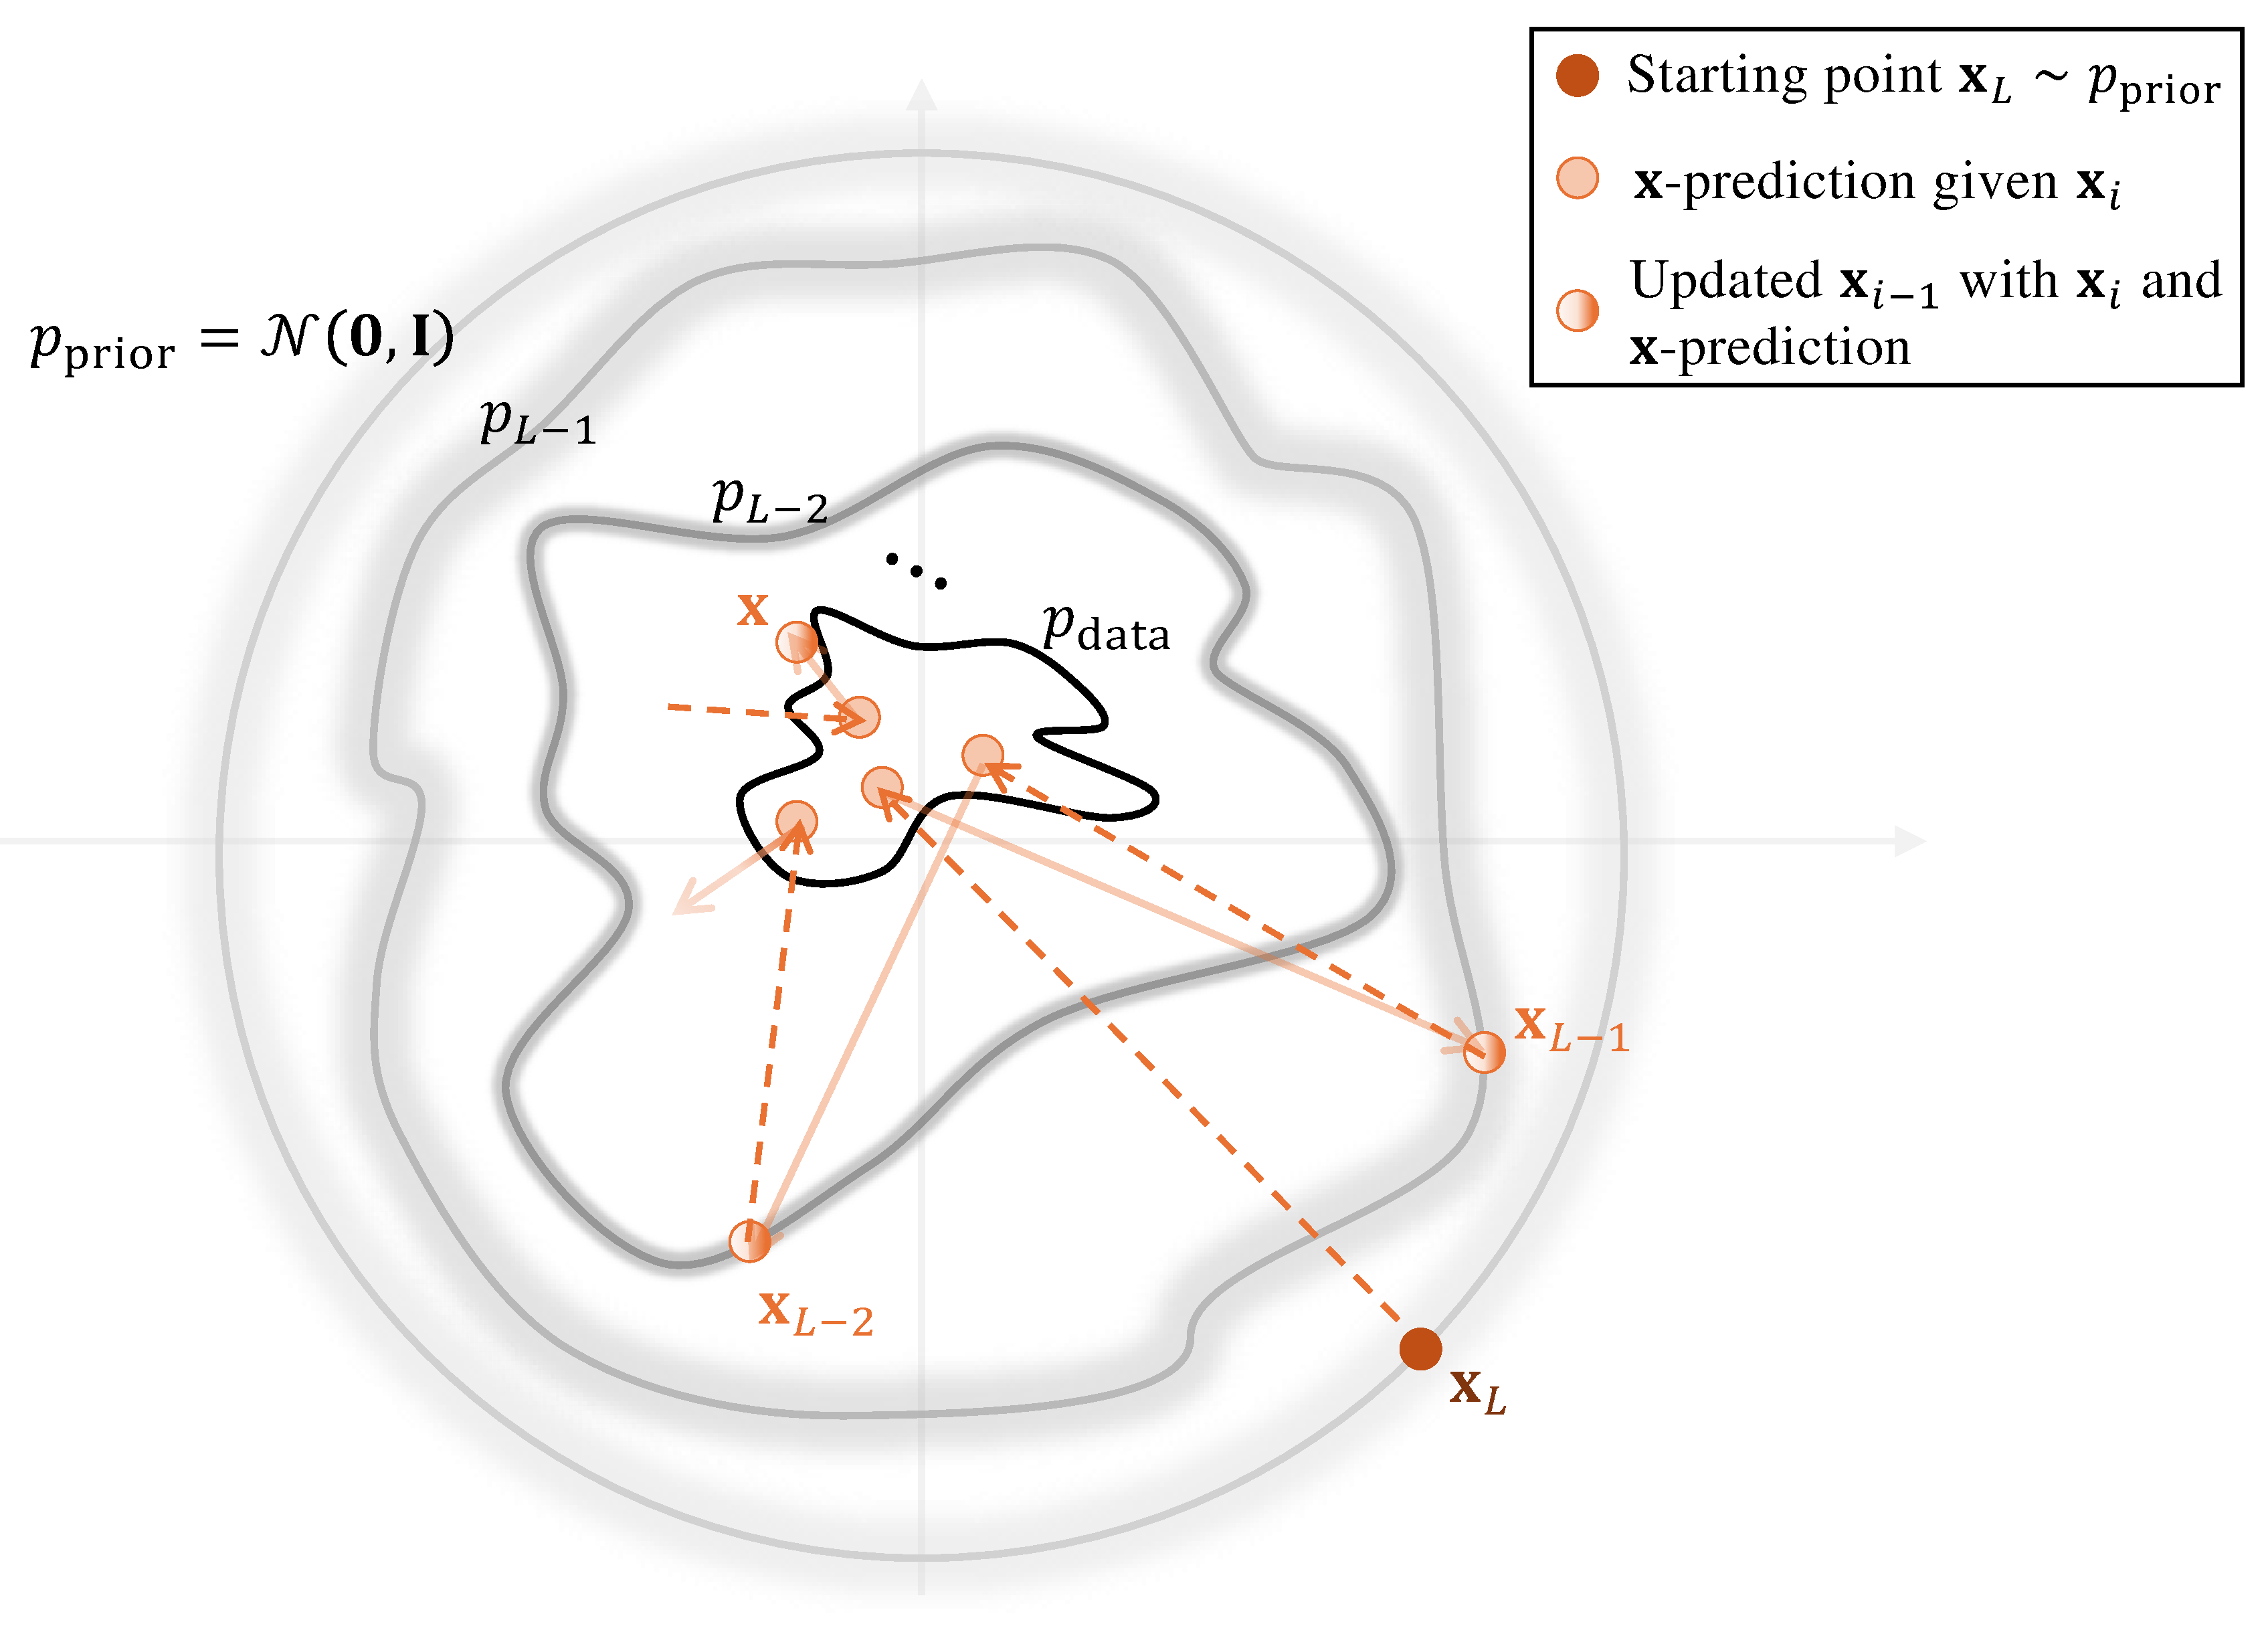
\includegraphics[width=\linewidth]{Images/PartB/diffusion-clean.pdf}
\caption{\textbfs{DDPM 采样“先去噪再重新加噪”视角的示意图。}
从当前噪声样本 $\mathbf{x}_i$ 出发，模型首先估计潜在的干净信号 $\mathbf{x}_{\bm{\phi}^\times}(\mathbf{x}_i,i)$，然后通过将该估计重新加噪至第 $(i-1)$ 个噪声水平来采样一个噪声更小的点 $\mathbf{x}_{i-1}$。\figcredit{由作者绘制。}}
    \label{fig:vdm-clean}
\end{figure}



\paragraph{DDPM 缓慢的采样速度。} DDPM（即扩散模型）的采样本质上是缓慢的。在原始的表述和实现中，生成一个样本通常需要大约 $1{,}000$ 个去噪步骤。这是因为采样通过一长串小的细化进行：在每一步，模型将当前噪声样本稍微向更干净的方向更新，而下一步更新必须从前一步的结果开始。因此，标准 DDPM 采样是时间步进的、强顺序的，而良好的样本质量通常需要许多这样的步骤来紧密跟踪反向扩散路径。

定理~\ref{thm:equiv-marginal-kl} 表明，一个富有表现力的 $ p_{\bm{\phi}}(\mathbf{x}_{i-1} | \mathbf{x}_i) $ 理论上能够匹配真实的反向分布 $ p(\mathbf{x}_{i-1} | \mathbf{x}_i) $。然而在实践中，$ p_{\bm{\phi}}(\mathbf{x}_{i-1} | \mathbf{x}_i) $ 通常被建模为高斯分布以近似 $ p(\mathbf{x}_{i-1} | \mathbf{x}_i) $，这限制了其表达能力。

对于较小的前向噪声尺度 $\beta_i$，真实反向分布近似为高斯分布，从而能够精确近似。相反，较大的 $\beta_i$ 会诱发单高斯无法捕捉的多峰性或强非高斯性。为了保持精度，DDPM 采用许多小的 $\beta_i$ 步骤，形成一条顺序链，其中每一步都依赖于前一步，并需要一次神经网络求值 $\boldsymbol{\epsilon}_{\bm{\phi}^\times}(\mathbf{x}_i, i)$。这导致 $\mathcal{O}(L)$ 次顺序传递，阻碍了并行化并拖慢了生成。



在后面的 \Cref{ch:score-sde} 中，我们将展示对这一固有采样瓶颈的一种更有原则的解释，即将其视为一个微分方程问题，这激发了用于加速生成的连续时间数值策略。



\newpage
\section{结语}\label{sec:ch2_cr}


在本章中，我们通过变分的视角追溯了扩散模型的起源。我们从变分自编码器（VAE）开始，它是一个基础的生成模型，通过证据下界（ELBO）学习数据与一个结构化隐空间之间的概率映射。我们看到层次化 VAE（HVAE）如何通过堆叠隐层来扩展这一思想，引入了渐进式、由粗到细生成的有力概念。然而，这些模型面临训练稳定性和样本质量方面的挑战。





然后，我们将去噪扩散概率模型（DDPM）构建为这一变分框架内的一次关键演进。通过将编码器固定为一个渐进的加噪过程并仅学习反向去噪步骤，DDPM 优雅地避开了 HVAE 的训练不稳定性。关键的是，我们证明了 DDPM 也是通过最大化对数似然上的一个变分界来训练的，其训练目标分解为一系列简单的去噪任务。这种可处理性由一种有力的条件化策略促成，该策略将一个不可处理的边际目标转化为一个可处理的条件目标，这是扩散模型中反复出现的主题。





虽然这一变分框架为 DDPM 提供了一个完整而有力的基础，但它并不是理解它们的唯一方式。一种替代且同样基础的视角从基于能量的建模原理中涌现。在下一章中，我们将探讨这种基于分数的视角：
\begin{enumerate}
    \item 我们将把焦点从学习去噪转移概率 $p_{\bm{\phi}}(\mathbf{x}_{i-1}\vert\mathbf{x}_{i})$ 转移到直接学习数据对数密度的梯度，即分数函数。
    \item 我们将看到这一源于 EBM 的方法如何催生噪声条件分数网络（Noise Conditional Score Network，NCSN），并揭示 DDPM 中学到的噪声预测（$\bm{\epsilon}$-预测）与分数函数本身之间深刻的数学等价性。
\end{enumerate}

这一替代视角不仅将提供新的洞察，还将作为稍后开发的扩散模型统一连续时间框架的另一块基石。







